\pdfoutput=1

\pdfcompresslevel=1    % 1-9; 9 podczas rozwijania; 4 lub mniej do druku
\pdfobjcompresslevel=2
\pdfminorversion=7     % PDF 1.7 jest standardem ISO

\pdfinfo
{
    /Author (Adrian Pedziwiatr (180254))
    /Title (System do wzajemnej oceny kodu programistycznego)
}
\documentclass[a4paper,onecolumn,twoside,12pt]{mwrep}

%\usepackage{mathptmx}         % URW NimbusRomNo9L, odmiana Times New Roman, 
\usepackage{tgtermes}        % czcionka szeryfowa TeX Gyre Termes, nie powoduje problemów podczas kopiowania tekstu z PDF

\usepackage[utf8]{inputenc}  % kodowanie dokumentu
\usepackage[T1]{fontenc}     % system kodowanie czcionek
\usepackage[polish]{babel}   % niezbędne dla narodowych znaków
\usepackage{polski}          % polski słownik łamania wyrazów
\usepackage{geometry}        % możliwość ustawienia marginesów

\usepackage{csquotes}        % cudzysłowy; nie ma domyślnie ustawień dla języka polskiego
\DeclareQuoteAlias{croatian}{polish} % cudzysłowy dla Polski są takie jak w~Chorwacji

\usepackage{pdflscape}       % możliwość zmiany orientacji strony (landscape/portrait mode)
% bibliografia
% backend=biber
% backend=bibtex,bibencoding=ascii
\usepackage[
    backend=biber,
    natbib=true,
    style=numeric,
    sorting=nyt % sortowanie: nazwiska (n), rok (y), tytuł (t)
]{biblatex}
\addbibresource{999bibliografia.bib}

\hyphenpenalty=10000		% nie dziel wyrazów zbyt często
\clubpenalty=10000			% kara za sierotki
\widowpenalty=10000			% nie pozostawiaj wdów
\brokenpenalty=10000		% nie dziel wyrazów między stronami
\exhyphenpenalty=999999		% nie dziel słów z~myślnikiem
\righthyphenmin=3			% dziel minimum 3 litery

\pretolerance=250           % tolerancja dzielenia wyrazów (-1 do 10000)
\hbadness=10000             % zgłaszaj błędy 'underfull' 'overfull' (0 do 10000)
\sloppy						% umacnia pozycję prawego marginesu

\linespread{1.3}            % interlinia

\usepackage{graphicx}       % rysunki
\graphicspath{ {images/} {images2/} {db/} }  % źródło rysunków

\begin{document}
    \newgeometry{tmargin=2.5cm, bmargin=2.5cm, lmargin=2.5cm, rmargin=2.5cm}
    
    \begin{titlepage}
	\begin{center}
	\fontsize{12pt}{14pt}\selectfont
	Politechnika Łódzka \\
	Wydział Elektrotechniki, Elektroniki, Informatyki i~Automatyki \\
	Instytut Informatyki Stosowanej \\

	\vspace{3 cm}
	
	\fontsize{13pt}{28pt}\selectfont
    \textbf{PRACA DYPLOMOWA INŻYNIERSKA} \\
    System do wzajemnej oceny kodu programistycznego \\
    A~system for peer review of application source code \\
    
    \vspace{3 cm}

    \fontsize{12pt}{14pt}\selectfont
    Autor: Adrian Pędziwiatr \\
    Number albumu: 180254 \\
    
	\vspace{4 cm}
	
    \begingroup\raggedleft
	Opiekun pracy:\\
	dr inż. Radosław Adamus\par
    \endgroup

	\par\vspace*{\fill}
	Łódź, styczeń 2016

	\end{center}
\end{titlepage}


% ex: set tabstop=4 shiftwidth=4 softtabstop=4 noexpandtab fileformat=unix filetype=tex spelllang=pl,en spell:

    \null
    \thispagestyle{empty}
    \clearpage
    
    \newgeometry{tmargin=2.5cm, bmargin=2.5cm, lmargin=3.5cm, rmargin=2.5cm} 
    % streszczenie
\begin{center}
\addcontentsline{toc}{chapter}{\numberline{}Streszczenie}
\textbf{Streszczenie}
\end{center}

W ramach niniejszej pracy inżynierskiej autor opracował system do wzajemnej oceny kodu programistycznego. System ten nie jest kolejnym typowym systemem wspomagającym słownikowo rozumiany przegląd koleżeński. Zrealizowany system ma na celu dostosowanie wspomnianego przeglądu do realiów dydaktycznych.

Realizując specyficzne wymagania takie jak anonimowość przeglądu, czy nadzór osoby prowadzącej kurs (i~powierzenie jej roli zleceniodawcy), wspomagany przegląd oddalił się od definicji tytułowego przeglądu wzajemnego. Autor jest głęboko przekonany, iż realizacja przeglądów prac podczas nauki, nie tylko przez prowadzącego kurs, ale także przez kolegów pozytywnie wpłynie na skuteczność usuwania defektów i~postęp nauki. System ten ma to umożliwić.

System został zrealizowany jako aplikacja webowa. Jego budowanie przyświecała idea wielokrotnego użycia. W~tym celu system głęboko integruje się z~powszechnie wykorzystywanym systemem kontroli wersji Git, oraz usługą GitHub. Prowadzący kurs nie tylko nie musi rezygnować z~wykorzystywanych już narzędzi, ale także bezproblemowo może poszerzyć warsztat narzędzi dydaktycznych.

\vspace*{\baselineskip}

\noindent\textbf{Słowa kluczowe:} \textit{przegląd koleżeński, wielokrotne użycie}

\vspace*{1.5\baselineskip}

\begin{center}
\addcontentsline{toc}{chapter}{\numberline{}Abstract}
\textbf{Abstract}
\end{center}

Within this thesis the author has developed and implemented a~system for peer review of~application source code. This is not another system that just supporting peer review as~understood in~the~dictionary. System has been adapted to~the~realities of~learning process in~schools.

By~carrying out specific requirements such as \textquote{review must be anonymous} or \textquote{review is supervised by~the~person leading the course}, assisted review move away from the definition. The author is deeply convinced that performing peer review while learning, not only by course leader, but also by colleagues positively affect the efficiency of removal of defects and will speed up learning courve. This system is to create opportunities.

The system has been implemented as~a~Web application. Software reusable is~very important in that system. It deeply integrates with one of~commonly used version control system - Git and a~GitHub service. Course leader can easily start using this system and does not have to give up already using tools.

\vspace*{\baselineskip}

\noindent\textbf{Keywords:} \textit{peer review, reusability}


% ex: set tabstop=4 shiftwidth=4 softtabstop=4 noexpandtab fileformat=unix filetype=tex spelllang=pl,en spell:

    \clearpage
    \null
    
    \tableofcontents
    
    \chapter{Wstęp}

\section{Cel pracy}
Pomysłem przewodnim tej pracy inżynierskiej jest: studenci piszą programy - studenci je oceniają. Celem pracy jest opracowanie systemu, który umożliwia anonimowe przeglądanie kodu, przez kogoś równorzędnego do autora oraz dokonywanie oceny kodu na podstawie wytycznych zdefiniowanych przez zlecającego przegląd. Zakres pracy obejmuje projekt i~implementację systemu, oraz opisanie rezultatów pracy.

\section{Rodzaje przeglądów}
Przegląd kodu (ang. review) można podzielić na dwie zasadnicze kategorie:

\begin{itemize}
\item przegląd formalny (ang. formal review) - wysoce sformalizowany przegląd, prowadzony i~dokumentowany zgodnie z~ustaloną procedurą;
\item przegląd nieformalny (ang. informal review, ad-hoc review) - przegląd, którym nie kierują żadne formalne procedury.
\end{itemize}

Przeglądów nieformalnych tak na prawdę dokonujemy często - nie zastanawiając się na tym, a~nawet no tym nie wiedząc. Najprostszym przykładem przeglądu nieformalnego jest poproszenie kolegi o~pomoc w~rozwiązaniu problemu. Jednym z~typów przeglądu nieformalnego jest przegląd koleżeński. Adam Roman w~swojej książce pojęcie to definiuje następująco:

\medskip
\textquote{przegląd koleżeński (ang. peer review) - przegląd produktów powstałych podczas wytwarzania oprogramowania prowadzony przez kolegów ich twórcy mający na celu wskazanie defektów i~możliwości poprawek} \cite{TestPWN}

\medskip
Zwyczajowo przeglądy wykonuje się w~pracy zawodowej, starając się zapewnić jak najwyższą jakość tworzonego oprogramowania. Działający produkt to nie wszystko. Każde oprogramowanie dostarczające rozwiązanie niebanalnego problemu posiada błędy. Ważne jest, aby te błędy wykrywać jak najszybciej. Im szybciej wykryta i~naprawiona zostanie usterka, tym mniejszy koszt wygeneruje. Przeglądy są jednym z~typów testowania statycznego, których celem jest jest odnajdywanie defektów na jak najwcześniejszym etapie. Mediana skuteczności usuwania defektów przy wykonywaniu przeglądu wynosi około 60\% dla przeglądów formalnych, i~około 35\% dla przeglądów nieformalnych \cite{TestPWN}. Statystyki te zachęcają do przyjrzenia się bliżej przeglądom i~wykorzystaniu ich potencjału nie tylko w~czasie pracy zawodowej.

\section{Cel biznesowy}
Przegląd koleżeński jest tym typem przeglądu na którym skupiono się w~tej pracy. Motywacją, która przyświeca tej pracy jest uwzględnienie takiej czynności w~procesie nauki. Nie da się nauczyć tworzyć dobre oprogramowanie kończąc na realizacji algorytmu. Refaktoryzacja działającego kodu jest ważnym etapem. O~wiele prościej jest ją wykonać, gdy ktoś da nam wskazówki, przedstawi swoje uwagi. Te natomiast łatwo zdobyć wykonując przegląd koleżeński.

\medskip
System zaprojektowano z~myślą o~zajęciach studenckich, na których prowadzący laboratoria może zadać studentom jako formę ćwiczenia wykonanie przeglądu prac swoich kolegów. Przegląd taki wykonywany jest według kryteriów ustalonych przez prowadzącego i~jest anonimowy (oceniający nie zna autora pracy). Na potrzeby procesu zbierania wymagań, a~później projektowania systemu, zajęcia studenckie zostały uogólnione do postaci kursu, a~studenci do kursantów. W~kontekście systemu laboratoria studenckie nie wyróżnia nic, co by nakazywało użyć formy bardziej szczegółowej. Ponadto takie określenia zaznaczają, że system jest uniwersalny i~może być użyty nie tylko w~ramach zajęć studenckich, lecz w~trakcie jakichkolwiek kursów związanych z~nauką programowania.


% ex: set tabstop=4 shiftwidth=4 softtabstop=4 noexpandtab fileformat=unix filetype=tex spelllang=pl,en spell:

    \chapter{Wymagania}

\section{Cel systemu}

Wymagania stawiane systemowi do wzajemnej oceny kodu, wykorzystywanemu w~procesie nauki są inne niż przypadku pracy zawodowej. Celem systemu jest spowodowanie, aby kursant-recenzent przyjrzał się pracy wykonywanej przez innych kursantów. Pozwoli mu to spojrzeć na kod z~innej perspektywy. Możliwe jest, że wtedy zauważy inne elementy, rozważy nowe sposoby rozwiązania, nauczy się czegoś. System, który spełni postawione wymagania potencjalnie może wspierać wiele scenariuszy. Osoba oceniającą może być zarówno \textquote{poprowadzona za rękę} poprzez przekazanie jej podczas procesu oceny szczegółowych instrukcji, jak i~pozostawiona sama sobie posiadając jedynie ogólne wskazówki i~pytania.

\section{Aktorzy systemu}
System musi uwzględniać następujące role:

\begin{itemize}
    \item prowadzący kurs (ang. course master),
    \item zleceniodawca przeglądu (ang. review supervisor),
    \item uczestnik kursu (ang. course partiticipant),
    \item autor pracy, osoba oceniana (ang. assessed person),
    \item recenzent, osoba oceniająca (ang. reviewer, assessor).
\end{itemize}

\section{Cechy systemu}
System wykonany w~ramach niniejszej pracy inżynierskiej, w~porównaniu do tradycyjnych systemów wspomagających proces przeglądów nieformalnych, wyróżnia się w~następujących elementach:

\begin{itemize}
    \item przegląd zleca osoba nadrzędna (zleceniodawca),
    \item oceniana jest całość, nie pojedyncza zamiana,
    \item ocena następuje poprzez wypełnienie ankiety,
    \item ocena następuje według określonych kryteriów,
    \item ocena jest dokonywana anonimowo.
\end{itemize}

Różnice wynikają z~innej grupy docelowej, która ma system wykorzystywać, i~celom, którym ma służyć. Jest to jednocześnie spis wymagań postanowionych w~stosunku do tworzonego oprogramowania, które zostały przewidziane i~zrealizowane.

\subsection{Zleceniodawca przeglądu}
Wykorzystując system wspomagający przegląd koleżeński w~zakładzie pracy zleceniodawcą przeglądu może być zarówno kierownik, jak i~pracownik (chociaż z~definicji należało by mówić tylko o~koledze - pracowniku). Wybór osoby oceniającej także leży w~gestii obydwu tych osób. Wszystko zależy od tego, jakie są przyjęte w~firmie (projekcie) zasady, i~jaka jest motywacja przeglądu. Może tu chodzić zarówno o~sprawdzenie kodu osoby mniej doświadczonej, przez bardziej doświadczoną - gdzie głównym celem jest poprawa jakości kodu, jak i~odwrotnie - gdzie mimo świeżego poglądu prawdopodobnie większy zaobserwowany zysk będzie w~aspekcie edukacyjnym (zobaczeniu jak pewne problemy rozwiązują starsi, bardziej doświadczeni koledzy).

\medskip
W opracowanym systemie przegląd jest rodzajem ćwiczenia, w~szczególnym przypadku pracy domowej. Wykonanie przeglądu zawsze zleca osoba nadrzędna - prowadząca kurs. W~chwili obecnej nie przewidziano możliwości wskazania kto ma czyją pracę ocenić - jako element nieistotny przydział został zrealizowany losowo, jednak z~uwzględnieniem tego, że powinien być równomierny - tj. każda praca oceniona tyle samo razy.

\subsection{Ocena całości}
W typowym systemie często nie chodzi o~przegląd całej aplikacji - gdyż jest to często niemożliwe z~uwagi stopień jej skomplikowania. Osoba nr 1 implementując nową funkcjonalność, lub modyfikując istniejącą potencjalnie eliminuje, lub wprowadza nowe błędy w~systemie. Motywacją przeglądu kodu przez inną osobę (nr 2) jest między innymi jest poprawienie jakości tego kodu, eliminacja defektów, skupiając się na tym, co zostało w~nim zmodyfikowane. Historia zmian jest istotną kwestią w~tej motywacji.

\medskip
W opracowanym systemie historia zmian nie jest istotna. Z~założenia program nie jest długi, a~osoba oceniająca nie musi znać historii, wiedzieć jak wyglądał rozwój. Ważny jest efekt końcowy - i~to on powinien zostać oceniony, w~całości.

\subsection{Sposób oceny}
Typowy system zwykle umożliwia napisanie komentarza: do linijki kodu, do funkcji, do pliku, do całej ocenianej zmiany. Nie ma tu jednak żadnej standaryzacji. Każdy wpisuje swoje uwagi w~miejscu, które uważa za najodpowiedniejsze. Zwykle wybór ten zależy od tego, jak bardzo szczegółowa uwaga zostaje zanotowana. Trudno więc porównać otrzymane uwagi, w~przypadku gdy ten sam fragment przegląda wiele osób. 

\medskip
W opracowanym systemie recenzent nie wpisuje oceny bezpośrednio komentując kod. Prowadzący może określić zarówno szczegółowe kryteria jak i~dać jedynie ogólne wskazówki/pytania. Ważne jest, by możliwe było łatwe porównanie opinii różnych uczestników kursu na daną realizację zadania (w~przypadku, gdy pracę oceniało wiele osób). Ustalonym sposobem oceny spełniających to wymaganie jest wypełnienie przez recenzenta odpowiednio przygotowanej ankiety. Ankietę przygotowuję prowadzący uwzględniając co było w~danym zadaniu ważne, jaki scenariusz chciałby zrealizować, oraz jaki cel chciałby osiągnąć w~tym ćwiczeniu. Ankieta jako sposób oceny daje szeroką gamę możliwości i~czyni system bardziej wszechstronnym.

\subsection{Kryteria oceny}
W typowym systemie kryteria oceny mogą dotyczyć zgodności napisanego kodu z~zasadami przyjętymi w~firmie - dla przykładu: stosowane formatowanie kodu, unikanie niezalecanych funkcji. Każdy przegląd jest jednak inny, dotyczy czegoś innego - brak jest formalnej procedury. 

\medskip
W opracowanym także można przygotować ogólny zestaw pytań, pasujący do każdego zadania. Typowy przebieg jest w~nim jednak inny. Tutaj proces oceny dotyczy wcześniej przygotowanego, dokładnie przemyślanego zadania. W~zamyśle prowadzącego kurs było ułożenie tego zadania tak, by np. zasadnym było wykorzystanie konkretnego wzorca programistycznego. Łatwo jest przygotować wyspecjalizowane kryteria oceny, którymi powinien podążać recenzent. Punkt ten naturalnie związany jest ze sposobem oceny i~uzupełnia wymóg dostosowania sposobu oceny.

\subsection{Anonimowość przeglądanej pracy}
Typowa ocena jest imienna - to znaczy nie ma powodu, by ukrywać informację kto jest autorem ocenianej pracy. Realizowany system zakłada jednak, że uczestnik kursu nie wie czyją pracę ocenia. Anonimowe przedstawienie pracy zapewnia, że recenzent nie będzie się sugerował faktem, iż ocenia osobę, której wyniki są zwykle powyżej lub poniżej przeciętnej. Taka autosugestia może negatywnie wpłynąć na bezstronność oceny, szczególnie na etapie nauki. Dlatego też system zapewniać musi, iż recenzent nie zostanie poinformowany o~personaliach autora kodu.


% ex: set tabstop=4 shiftwidth=4 softtabstop=4 noexpandtab fileformat=unix filetype=tex spelllang=pl,en spell:

    \chapter{Potencjał do badań naukowych}
Wymagania postawione przed systemem, w~celu zrealizowania określonego celu biznesowego, jasno ukazują, że opracowany system odbiega od definicji \textquote{przeglądu nieformalnego}, jakim jest tytułowy \textquote{przegląd koleżeński}. Odstępstwa, takie jak wprowadzenia procedury oceny, czy wymuszenie tej oceny przez wydanie polecenia osoby nadrzędnej, skłaniają ku klasyfikowaniu go jako "przeglądu formalnego". Trudno jednak wskazać bez wątpliwości jego klasyfikację. System ten jest swego rodzaju hybrydą rozwiązań opisanych już w~książkach, i~zbadanych pod kątem skuteczności.

\medskip
Wniosek ten zachęca do przeprowadzania badań nad skutecznością takiego mieszanego rozwiązania. Nie tylko w~kwestii skuteczności wykrywania defektów, ale także w~kontekście zyskiwanych umiejętności. Warto sprawdzić, czy istnieje zależność pomiędzy tym, że kursanci regularnie oceniali w~ten sposób prace kolegów, a~ich wynikami w~kursie. Potencjalnym zyskiem może być też spłaszczenie krzywej nauki, szybsze nabieranie właściwych nawyków czy staranniejsze wykonywanie zadań, z~uwagi na sam fakt bycia ocenianym nie tylko przez prowadzącego kurs, ale także przez kolegów.

\medskip
Przeprowadzanie tego typu badań wykracza jednak poza zdefiniowany zakres pracy. Praca skupia się nad jak najlepszym zaprojektowaniem systemu, implementacją zgodną ze sztuką, oraz opisaniem zrealizowanego systemu.


% ex: set tabstop=4 shiftwidth=4 softtabstop=4 noexpandtab fileformat=unix filetype=tex spelllang=pl,en spell:

    \chapter{Sposób realizacji wymagań}

Wymagania nie wymuszają sposobu ich realizacji. W~czasie projektowania systemu autor przemyślał kilka rozwiązań i~ocenił pod kątem ich przydatności w~realizowanym systemie, trudności implementacji i~atrakcyjności biznesowej.

\section{Źródło ocenianych prac}
Pierwszą ważną kwestią jest źródło ocenianych prac. Prowadzący kurs mógłby na przykład udostępniać poprzez system zadanie do realizacji, a~kursanci po jego wykonaniu wgrywać rozwiązanie do systemu za pomocą odpowiedniego formularza. Takie rozwiązanie nie uzależnia od żadnych zewnętrznych usług. Problemy rodzi dopiero możliwość aktualizacji zadania, notowanie postępów w~czasie. Nie jest to także atrakcyjne wyjście z~biznesowego punktu widzenia.

\medskip
Wzorując się jednak na istniejących narzędziach zauważyć należy, że wykorzystują one do działania systemy kontroli wersji (ang. revision control system). Wykorzystanie takiego systemu nie koniecznie ułatwia implementację systemu. Znacząco usprawnia jednak prowadzenie kursów, zwłaszcza gdy dodatkowo wykorzystany zostanie usługa pozwalająca przechowywać repozytorium (ang. repository) systemu kontroli wersji (pliki, i~historię ich zmian) online. Kontrola wersji jest aktualnie nieodłącznym elementem programowania. Dlatego projektowany system w~znacznej części opiera się o~kontrolę wersji, i~usługi z~tym związane. Wybranym źródłem ocenianych prac jest usługa przechowująca historię wersji w~Internecie. Naturalnym wydaje się próba integracji z~już wykorzystywanymi usługami, ma to też uzasadnienie biznesowe.

\section{Sposób autoryzacji użytkownika}
Użytkownik musi mieć konto w~systemie, aby mógł zobaczyć zlecenia przeglądów, które zostały mu zadane, oraz na nie odpowiedzieć. Wymóg logowania zapewnia także, że nikt nie wypełni jego pracy. Klasycznym sposobem autoryzacji użytkowników jest założenie mu konta w~serwisie i~przekazanie danych autoryzujących, lub pozwolenie na samodzielne założenie konta (ewentualnie połączone z~automatycznym lub manualnym mechanizm potwierdzania prawidłowości wprowadzonych danych).

\medskip
Należy się jednak zastanowić, czy jest konieczne, aby kursant musiał mieć kolejne konto. W~związku z~założeniem, iż projekt opiera się na usługach związanych kontrolą wersji autor rozważył pogłębienie integracji. Usługi takie często oferują mechanizmy dostępu do zasobów prywatnych innym usługom, bez przekazywania danych autoryzujących. Przykładem takich sposobów autoryzacji są SAML, OpenID, OAuth1, OAuth2 \cite{3rdAuth}. Taki mechanizm łatwo wykorzystać jako sposób logowania za pomocą konta w~aplikacji trzeciej. Wystarczy, że wymagamy od kursanta posiadania konta w~usłudze związanej z~systemem kontroli wersji - nie ma potrzeby wymagać od niego jeszcze jednego konta. Rozwiązanie takie daje jeszcze jedną korzyść - brak konieczności dodatkowego łączenia pomiędzy kontem w~serwisie a~kontem w~usłudze kontroli wersji. 

\section{Anonimowość przeglądanej pracy}
Istotnym wymaganiem jest anonimowość przeglądanej pracy. Recenzent nie może wiedzieć, czyją pracę ocenia. Nie można więc po prostu mu przekazać adresu, gdzie autor umieścił swoje rozwiązanie. Przekazujemy w~ten sposób wszystkie meta-dane tam zawarte, w~tym autora pracy. Problem ten autor rozważył uwzględniając dodatkowe założenie integracji z~usługą kontroli wersji. Autor nie dokonał analizy technik możliwych do zastosowania w~przypadku innego źródła ocenianych prac.

\medskip
Jednym z~pomysłów rozwiązania tego problemu jest założenie kursantom kont prywatnych w~usłudze przechowywania repozytorium historii wersji. Każde takie konto może mieć nazwę, która nie musi zdradzać personaliów kursanta. Prywatne konta jednak częściowo nie spełniają wymagania, mówiącego, że ewentualne usługi trzecie muszą być darmowe. W~przypadku poziomu akademickiego często można poprosić o~takie konta, dla potrzeb uczelni. Chcąc jednak uogólnić system nie można przyjąć tego rozwiązania jako satysfakcjonującego.

\medskip
Innym, wykorzystanym, sposobem jest skopiowanie danej pracy, i~przekazanie recenzentowi kopii. Kopia taka, odpowiednio przygotowana, dokonana przy użyciu specjalnie do tego przeznaczonego konta, spełnia wymóg anonimowości. Autor widniejący pod przekazanym adresem nie odzwierciedla wtedy prawdziwej informacji, za każdym razem wskazuje na to samo bezosobowe konto.


% ex: set tabstop=4 shiftwidth=4 softtabstop=4 noexpandtab fileformat=unix filetype=tex spelllang=pl,en spell:

    \chapter{Wykorzystane technologie}

\section{Spis użytych technologii}
System został napisany jako aplikacja webowa, w~języku Java, w~wersji 1.8. Java to obiektowy, silnie typowany, wieloplatformowy język programowania, obecnie rozwijany przez firmę Oracle Corporation. Ponadto do realizacji systemu wykorzystano takie istniejące rozwiązania jak:

\begin{itemize}

\item Git - rozproszony system kontroli wersji (ang. version control system). System kontroli wersji pozwala śledzić zmiany w~dokumencie. Zapisuje on kto, kiedy i~jakie modyfikacje w~dokumencie dokonał. Programowanie jest dziedziną, gdzie systemy kontroli wersji wykorzystuje się powszechnie. Ułatwiają one pracę wielu osób nad jednym dokumentem, wycofywanie nieprawidłowych zmian, znalezienie winnego błędnej modyfikacji, czy proces przeglądu kodu \cite{PoCoKontrola}. W~programowaniu Git to jeden z~obecnie (2014) najpopularniejszych systemów kontroli wersji, zyskuje on na znaczeniu w~ostatnich latach (2011-2014) \cite{EclipseSurvey};

\medskip
\item GitHub - usługa internetowa, pozwalająca na przechowywanie repozytoriów Git. Oferuje całą bazową funkcjonalność systemu Git, a~także ją dodatkowo ją rozszerza. Z~usługi tej korzysta obecnie 12,4 mln osób, którzy rozwijają projekty w~ramach 31,7 mln repozytoriów systemu kontroli wersji \cite{GitHubPress}. Darmowe konto pozwala przechowywać nieograniczoną liczbę repozytoriów publicznych, do których można zaprosić nieograniczoną liczbę współautorów. Za możliwość utworzenia repozytorium prywatnego trzeba zapłacić;

\medskip
\item Gradle - system zarządzania zależnościami dla języka Java. Gradle jest alternatywną dla znacznie popularniejszych systemów takich jak Maven, czy Ant \cite{EclipseSurvey}. Autor dokonał wyboru systemu zarządzania zależnościami pomiędzy systemami Maven i~Gradle - systemy te są wspierane przez wybraną bazową platformę programistyczną (Spring Framework). Ostateczny wybór jest kwestią indywidualnych upodobań autora. Autor uważa, że składnia używana przez Gradle jest znacznie czytelniejsza niż w~Maven - w~szczególności lista zależności. System zarządzania zależnościami odpowiada za proces budowania do wybranego wspieranego formatu wynikowego, a~także za pobranie pakietów (plików .jar) zależności przed procesem budowania oprogramowania. Dzięki temu nie ma potrzeby dostarczania z~kodem źródłowym systemu także pakietów zależności - te zostaną pobrane automatycznie. System zarządzania zależnościami, we współpracy ze zintegrowanym środowiskiem programistycznym (ang. Integrated Development Environment, IDE), potrafi także pobierać dokumentacje i~kody źródłowe wykorzystywanych zależności - co znacząco podnosi komfort programowania;

\medskip
\item Spring Framework - platforma programistyczna (ang. framework) dla języka Java, dostarcza takie komponenty jak: szkielet wzorca architektonicznego Model-Widok-Kontroler (ang. Model-view-constoller, MVC), mechanizm wstrzykiwanie zależności, mechanizm zarządzania transakcjami, mechanizm zarządzania dostępem do danych i~inne. Platforma ta jest podstawą systemu. Definiuje ona główną architekturę systemu. Zastosowanie platformy z~reguły poprawia jakość pisanego kodu, podnosi efektywność procesu programowania, a~także zwiększa niezawodność systemu \cite{Framework}. W~zamian podnosi złożoność systemu, oraz może obniżyć jego wydajność \cite{Framework};

\medskip
\item Spring Boot - biblioteka dostarczająca strategię \textquote{konwencja, nie konfiguracja} (ang.~convention over configuration) dla platformy Spring. Jest to dodatkowa warstwa, która wykorzystuje jako zależność oryginalną platformę Spring Framework. Jej celem jest minimalizacja liczby konfiguracji wymaganej do uruchomienia strony internetowej z~wykorzystaniem platformy Spring. Biblioteka ta została wydana w~kwietniu 2014 roku, jako \textquote{recepta} na zbytnie skomplikowanie bazowej platformy Spring Framework, która wymaga dużej liczby konfiguracji~i szerokiej wiedzy na temat sposobu jej działania \cite{SpringIssueBoot}. Oficjalnym \textquote{zalążkiem} tej biblioteki jest zgłoszenie, w~systemie zgłaszania i~śledzenia błędów (ang. issue tracker) platformy Spring Framework,~w 2012 roku propozycji \textquote{improve support for 'containerless' web application architectures}, gdzie Mike Youngstrom opisał wady istniejącego rozwiązania i~zaproponował zmianę koncepcji \cite{SpringIssueBoot};

\medskip
\item Jetty - serwer stron internetowych i~serwletów języka Java, napisany w~całości w~tym języku. Może działać w~trybie wbudowanym (ang. embedded mode). Jeden z~dwóch, obok Tomcat, serwerów wspieranych przez Spring Boot. Autor wybrał ten serwer na podstawie własnych preferencji, kierując się głównie historią wersji obydwu serwerów, która wskazuje iż rozwój Jetty jest aktywniejszy, i szybciej podąża za nowymi technologiami;

\medskip
\item H2 - system zarządzania relacyjną bazą danych (ang. relational database management system, RDBMS). Jest napisany w~języku Java, wspiera standard SQL, charakteryzuje go wysoka wydajność w~trybie wbudowanym i~obsługa transakcji bazodanowych \cite{H2Performance}. Autor w~ramach pracy zdecydował się użyć bazy danych w~trybie wbudowanym. Pod względem wydajności wybrana baza z~sukcesem konkuruje z~konkurencją, także tą, która wymaga do działania serwera, tzn. działających w~trybie klient-serwer (ang.~client-server mode) \cite{H2Performance}. Autor nie rozważał możliwości użycia baz nierelacyjnych (typu NoSQL), ani baz obiektowych (ang. object database);

\medskip
\item Hibernate ORM - biblioteka dla języka Java dostarczająca mechanizm mapowania z~relacyjnego systemu bazodanowego na obiekty w~języku Java. Implementuje ona oficjalny standard mapowania relacyjno-obiektowego (ang. object-Relational Mapping, ORM) dla języka Java: Java Persistence API (JPA). Mechanizm mapowania relacyjno-obiektowego pozwala odwoływać się do danych, zapisanych w~bazie w~sposób relacyjny, w~sposób obiektowy z~poziomu języka programowania. Klasa reprezentująca tabelę w~bazie danych nazwa się encja (ang. entity). Za operację typu CRUD (ang. create, read, update, delete; pol. utwórz, odczytaj, aktualizuj, usuń) na warswie bazy danych odpowiada menadżer encji (ang. entity manager). Wykorzystanie ORM odciąża programistę od potrzeby pisania zapytań SQL (operowanie na encjach jest także bardziej naturalne dla programowania obiektowego), oraz zabezpiecza przed atakami typu \textquote{SQL injection};

\medskip
\item Thymeleaf - biblioteka dla języka Java dostarczająca silnik szablonów do przetwarzania i~generowania dokumentów HTML, XML, plików JavaScript, CSS. Pisany system jest dynamiczny. Informacje wyświetlane użytkownikowi zależą od aktualnego stanu systemu. Wykorzystanie silnika szablonów zapewnia wydzielenie warstwy widoku, zgodnie z~wykorzystanym wzorem model-widok-kontroler. Widok zawiera referencję do modelu, otrzymaną od kontrolera skąd może pobrać za każdym razem aktualne dane. Wybrany silnik szablonów posiada wsparcie dla najnowszej wersji standardu HTML (HTML5), internacjonalizacji oraz automatycznie kontroluje poprawność składniową generowanego dokumentu;

\medskip
\item OAuth2 - otwarty standard autoryzacji użytkowników. Określa on przebieg procesu dostępu do zasobów aplikacji trzeciej, bez udostępniania danych autoryzujących. Użytkownik w~systemie musi być autoryzowany. Ustalonym sposobem autoryzacji jest OAuth2, gdyż to właśnie ten sposób jest wpierany przez usługę GitHub;

\medskip
\item pac4j: Spring Web MVC / Spring Boot - biblioteka dla języka Java dostarczająca mechanizmy pozwalające zabezpieczyć systemy webowe przed dostępem osób nieautoryzowanych. Budowa tego mechanizmu jest modułowa. Dołączając odpowiedni można przy jej użyciu zrealizować właściwie każdy sposób uwierzytelnienia (ang. authentication) i~autoryzacji (ang. authorization) użytkownika;

\medskip
\item pac4j-oauth: moduł biblioteki pac4j pozwalający zrealizować system autoryzacji z~użyciem standardu OAuth2. W~projektowanej aplikacji rolę serwera autoryzacji (ang. authorization server) i~serwera zasobów (ang. resource server) pełni usługa GitHub;

\medskip
\item GitHub API v3 (GitHub API) - interfejs programistyczny pozwalający w~sposób programowy komunikować się z~usługą GitHub w~celu uzyskania lub modyfikacji zasobów, które one przechowuje. Interfejs programistyczny udostępniony przez GitHub jest bardzo zaawansowany. Można przy jego użyciu wykonać właściwie wszystkie akcje dostępne w~serwisie, w~tym te najbardziej interesujące w~kontekście budowanego systemu: odczyt podstawowych informacji na temat repozytorium (lista powieleń, lista gałęzi, nazwa gałęzi głównej, adres do pobrania repozytorium, możliwość utworzenia nowego);

\medskip
\item com.squareup: OkHttp - biblioteka dla języka Java, implementacja klienta http z~możliwością zapamiętywania odpowiedzi w~pamięci podręcznej (ang. cache);

\medskip
\item org.kohsuke: github-api - biblioteka dla języka Java będąca implementacją komunikacji z~GitHub API w~tym języku. Udostępniona dokumentacja API opisuje istniejące zasoby i~sposoby odwołania do nich. Nie istnieje jednak oficjalna implementacja dostępu do wspominanego API w~jakimś konkretnym języku programowania. Wybrana biblioteka udostępnia obiektowo-zorientowaną reprezentację komunikacji ze wspominanym API. Autor biblioteki deklaruje iż pokrywa ona \textquote{znaczną część} API. Autor sprawdził, iż pokrycie jest wystarczające do zrealizowana systemu;

\medskip
\item Eclipse JGit - biblioteka dla języka Java pozwalająca zarządzać repozytorium Git programowo, z~poziomu tego języka. W~opinii autora akcje takiej jak: zatwierdzanie zmian, synchronizacja repozytorium lokalnego ze zdalnym za pomocą GitHub API są mało intuicyjne i~stosunkowo trudne. Autor zdecydował się użyć innej biblioteki do tych zadań. Wybrana biblioteka JGit realizuje te zadania wykorzystując system plików - działa podobnie jak program \textquote{git}. Jest to biblioteka generyczna - znajduje zastosowanie zarówno dla repozytoriów lokalnych, jak i~dla~dowolnej usługi przechowującej repozytorium Git zdalnie;

\medskip
\item Apache POI - biblioteka dla języka Java, umożliwia generowanie dokumentów pakietu Microsoft Office (w~tym arkuszy Excel) programowo, z~poziomu tego języka. Podsumowania przeglądów system generuje jako arkusz MS Excel. Zastosowana biblioteka potrafi generować zarówno starsze pliki pakietu Office (przed wersją 2007), jak i~nowsze (od wersji 2007, z~dodatkową literą \textquote{x} w~rozszerzeniu);

\end{itemize}

\section{Wielokrotne użycie}
Wymyślanie koła na nowo nie zawsze jest dobrym rozwiązaniem. Pisaniu aplikacji sprzyjała idea wielokrotnego użycia. Wykorzystano jak najwięcej istniejących rozwiązań, w~większości znanych i~dojrzałych. Istotnym założeniem projektowania była integracja z~istniejącymi i~powszechnie wykorzystanymi usługami.
 
\subsection{Git i~GitHub}
System kontroli wersji Git, i~usługa GitHub odgrywają w~projekcie kluczową rolę. Oparte na tym zostało wiele elementów: system logowania, system anonimizacji ocenianych prac, prezentacja ocenianej pracy.

\medskip
Wyborowi systemu kontroli wersji Git sprzyjała głównie jego rosnąca popularność \cite{EclipseSurvey}, jak i~dostępność darmowych usług pozwalających przechowywać historię, zapisaną w~tym systemie, w~sieci internet.

\medskip
Na wybór usługi GitHub jako miejsca składowania kodu wpływ miał głównie fakt, iż udostępnia ona programistyczne API pozwalające sprawnie sprawdzić zasoby tego serwisu z~poziomu kodu, oraz może pełnić rolę serwera autoryzacji OAuth2. Pod uwagę autor wziął także dwa inne darmowe serwisy. Konkurencyjna usługa GitLab wykazuje poważne braki w~tych wymaganiach - udostępnia API, lecz nie wszystkie informacje o~zasobach, istotne z~punktu tworzonego systemu, są dostępne w~ten sposób \cite{GitLabApiDoc}. Inną konkurencyjną usługą jest Bitbucket, ten jednak nie jest chętnie używany z~uwagi na mało intuicyjny interfejs~\cite{GitOrBit}.

\subsection{Sposób uwierzytelnienia - OAuth2}
Użytkownik nie posiada oddzielnego konta w~systemie. Jego uwierzytelnienie następuje następuje z~użyciem usługi GitHub. Rozwiązanie takie nie tylko ma sens biznesowy (co autor udowodnił podczas opisu sposobu realizacji wymagań), ale także odciąża programistę i~administratora systemu od obowiązku zapewnienia przechowywania haseł w~sposób bezpieczny. Co prawda system wciąż przechowuje dane osobowe (imię i~nazwisko, powiązanie z~kontem GitHub), jednak poziom wrażliwości danych ulega obniżeniu. 

\medskip
Zastosowanym sposobem autoryzacji jest protokół OAuth2. Kluczowym elementem mający wpływ na wybór technologii autoryzacji było wsparcie jej przez usługę GitHub. Protokół OAuth2 określa sposób dostępu do zasobów usługi trzeciej (w~tym wypadku usługi GitHub) bez udostępniania danych autoryzujących (w~tym przypadku hasła w~usłudze GitHub). Uzyskane zezwolenie dostępu do zasób łatwo wykorzystać jako sposób uwierzytelnienia w~systemie. W~tym celu jedynym zasobem wykorzystywanym systemie jest nazwa użytkownika, który dostępu udzielił.

\medskip
Protokół OAuth2 definiuje następujące role:
\begin{itemize}
    \item właściciel zasobu (ang. resource owner) - użytkownik będący właścicielem zasobu. W~tym przypadkiem zasobem jest nazwa użytkownika, a~uwierzytelniany użytkownik jej właścicielem;
    
    \item klient (ang. client) - serwis, który chce poznać zasób. W~tym przypadku projektowany system chce poznać nazwę użytkownika w~usłudze serwera zasobów;
    
    \item serwer zasobów, dostawca API (ang. resource server) - usługa, do której dostęp należy uzyskać, aby zapoznać się z~zasobem. W~tym przypadku jest to usługa GitHub;
    
    \item serwer autoryzacji, dostawca tożsamości (ang. authorization server) - usługa, która udziela klucze dostępu do zasobów. W~tym przypadku nie ma wydzielonej takiej roli. Za czynność tą odpowiada sama usługa GitHub.
\end{itemize}

\medskip
Ponadto w~omawianym protokole występują dwa ważne pojęcia:
\begin{itemize}
    \item zgoda na dostęp (ang. authorisation grant) - potwierdzenie właściciela zasobu, że udziela klientowi dostępu do niego.
    \item token (ang. access token) - klucz, za pomocą którego  klient może przeczytać zasób u~dostawcy zasobu.
\end{itemize}

\medskip
Proces uwierzytelnienia w~wykorzystanym protokole wygląda następująco:
\begin{enumerate}
    \item użytkownik otwiera system. W~tym momencie nie jest zalogowany. Klikając odpowiedni przycisk stwierdza chęć autoryzacji z~użyciem określonego serwisu;
    \item użytkownik opuszcza system - zostanie przekierowany do serwera autoryzacji. Jedynym dostępnym serwisem uwierzytelniającym w~systemie jest usługa GitHub. W~tym momencie system przyjmuje rolę klienta, a~usługa GitHub serwera autoryzacji;
    \item użytkownik dowiaduje się od serwera autoryzacji, jaki klient prosi o~zgodę na dostęp i~do jakiego zasobu. Użytkownik potwierdza wydając zgodę na dostęp;
    \item użytkownik opuszcza serwer autoryzacji - zostaje przekierowany z~powrotem do systemu. W~sposób dla niego transparentny przekazuje do systemu token, który otrzymał od serwera autoryzacji. W~praktyce potwierdzając dostęp wysyła on formularz, kierujący do systemu, gdzie w ukrytym polu przekazywany jest wspomniany token;
    \item system odwołuje się do serwera zasobów, gdzie za pomocą tokena uzyskuje dostęp do zasobu, o~który prosił. System poznał w~tym momencie nazwę użytkownika i~posiada wszystkie dane by wykonać autoryzację i~określić uprawnienia użytkownika, który właśnie się zalogował. Użytkownikowi zostaje wyświetlony widok zgodny z jego rolą i uprawnieniami.
\end{enumerate}

\clearpage
Ilustracja technicznego przebiegu uwierzytelnienia z~użyciem protokołu OAuth2 została załączona jako rysunek \ref{obr13}.

\begin{figure}[!h]
\centering
    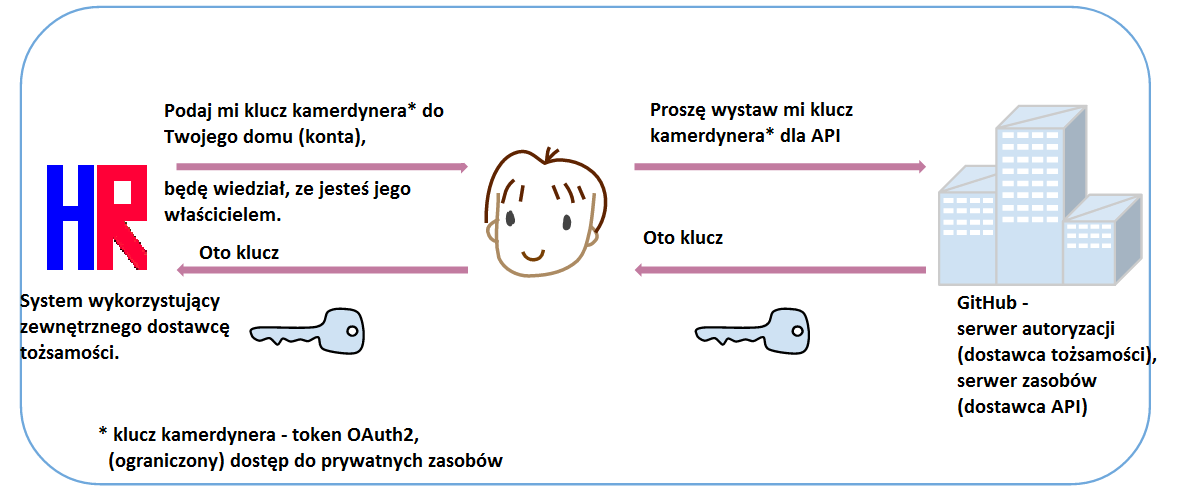
\includegraphics[width=\textwidth]{1_3oauth2}
    \caption[Przebieg uwierzytelnienia z~użyciem protokołu OAuth2]{Przebieg autoryzacji z~użyciem protokołu OAuth2. (Tłumaczenie własne zasobów Wikimedia Commons. Plik udostępniony na licencji Creative Commons CC0 1.0 Uniwersalna Licencja Domeny Publicznej. Pierwotni autorzy: Saqibali, Amada44, Perhelion.)}
    \label{obr13}
\end{figure}


\subsection{System formularzy}

System formularzy autor napisał na nowo, mimo iż istnieje wiele systemów tego typu. Podstawowym wymaganiem w~stosunku do systemu formularzu był dostęp do programistycznego API, który pozwoli założyć, kasować i~odczytywać historię odpowiedzi z~poziomu kodu. Usługa musiała być też darmowa, lub udostępniać darmowy dostęp do celów akademickich. Przetestowano wiele rozwiązań, jednak żadna z~nich nie była satysfakcjonująca dla potrzeb tego projektu. Z~tego autor powodu zdecydował się napisać prosty autorski system formularzy, dopasowany na miarę do realizowanego systemu.

% ex: set tabstop=4 shiftwidth=4 softtabstop=4 noexpandtab fileformat=unix filetype=tex spelllang=pl,en spell:


    \chapter{Architektura systemu}

System został napisany jako aplikacja webowa z~użyciem wzorca architektonicznego Model-Widok-Kontroler (ang. Model-View-Controller, MVC). Wzorzec ten zakłada podział aplikacji na 3 części:

\begin{enumerate}
\item model (ang. model) - który odpowiada za dane i~logikę biznesową;
\item widok (ang. view) - który odpowiada na interfejs, za pomocą którego użytkownik komunikuje się z~aplikacją;
\item kontroler (ang. controller) - który odpowiada za interakcję z~użytkownikiem, przyjmuje od niego dane wejściowe (przekazane za pomocą widoku), przetwarza informacje a~następnie aktualizuje model i/lub widok;
\end{enumerate}

\begin{figure}[!h]
\centering
    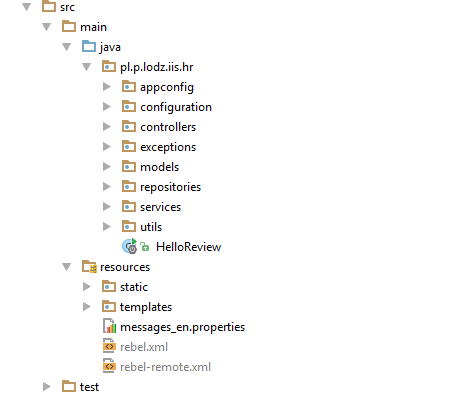
\includegraphics[width=360px]{0_1struktura}
    \caption{Architektura systemu - struktura plików}
    \label{obr01}
\end{figure}

\clearpage
Rysunek \ref{obr01} przedstawia strukturę plików w~projekcie. System składa kolejno z~takich pakietów jak:

\begin{itemize}

\item appconfig - zawiera klasy odpowiedzialne za odczyt z~pliku konfiguracji systemu; 

\item configuration - zawiera klasy odpowiedzialne za skonfigurowanie systemu, to znaczy skonfigurowanie bazowej platformy Spring Boot, połączenie z~nią używanych zależności (innych technologii), konfigurację serwera http;

\item controllers - klasy wchodzące w~skład warstwy kontroler. Odbierają żądania http, przekazują komunikaty do modelu, i~renderują odpowiedni widok zawierający odpowiedź;

\item exceptions - wydzielona część warstwy kontroler. Zawiera deklaracje klas odpowiedzialnych za obsługę sytuacji wyjątkowych;

\item models - część warstwy model. Zawiera encje - klasy odpowiadające za składowanie danych;

\item repositories - część warstwy model. Warstwa pośrednia pomiędzy sterownikiem dostępu do bazy danych, a~encjami. Zawiera, zgodnie ze wzorem repozytorium (ang. repository pattern), klasy umożliwiające operacje typu CRUD (utwórz, odczytaj, zaktualizuj, usuń; ang: create, read, update, delete), oraz operacje selekcji warunkowych w~systemie bazodanowym;

\item servives - część warstwy model. Zawiera usługi operujące na encjach, w~praktyce ten pakiet zawiera logikę biznesową;

\item utils - dodatkowe klasy narzędziowe, nie związane bezpośrednio z~aplikacją, lecz użyteczne przy jej tworzeniu;

\item resources/static - część warstwy view. Zawiera wszystkie pliki statyczne, które nie zależą od kontekstu wykonania, takie jak: obrazki, pliki skryptów JavaScript, arkusze styli CSS;

\item resources/templates - część warstwy view. Zawiera szablony generowane dynamicznie, zależne od kontekstu, i~danych przekazanych do nich poprzez kontroler.

\end{itemize}

\clearpage
Zastosowana struktura pakietów trochę rozdrabnia ogólny podział, który jest zdefiniowany przez wzorzec MVC. Wynika to z~naturalnej tendencji do separacji klas, które łączy wspólna cecha oraz chęci tworzenia systemu warstwowego, o~prostej strukturze zależności. Szkic założonej architektury zawiera rysunek \ref{obr02}.

\begin{figure}[!h]
\centering
    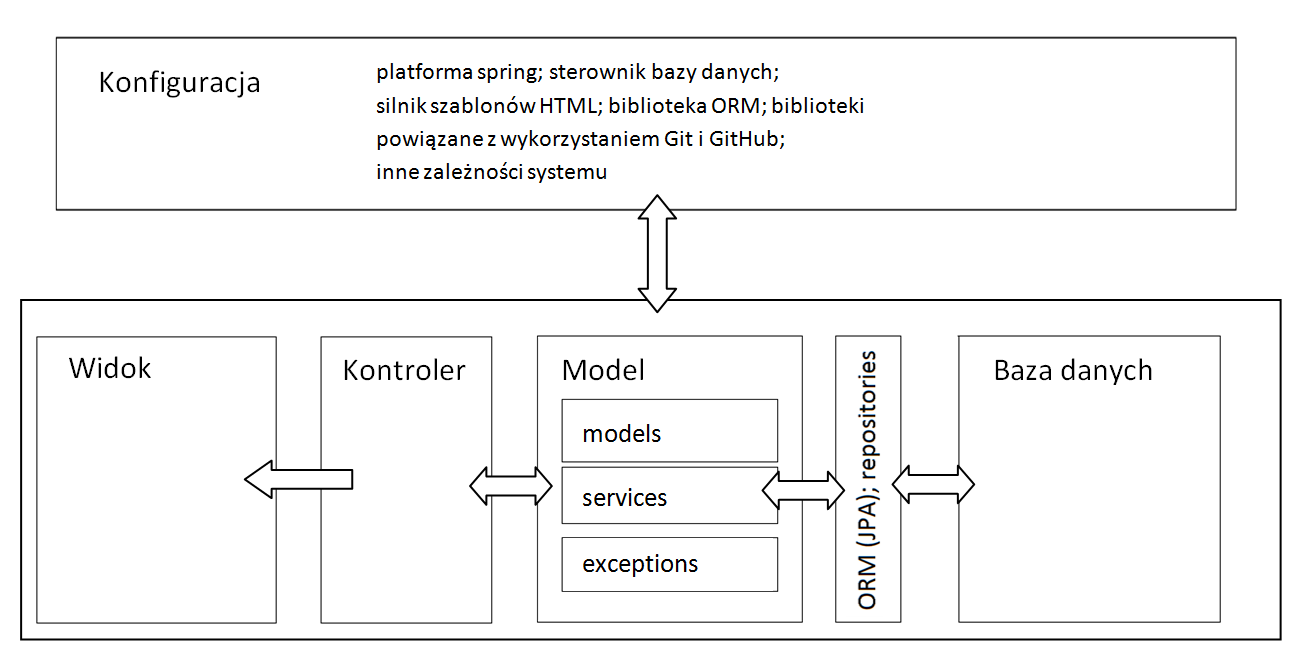
\includegraphics[width=\textwidth]{0_2architektura}
    \caption{Architektura systemu - zależność pakietów}
    \label{obr02}
\end{figure}

% ex: set tabstop=4 shiftwidth=4 softtabstop=4 noexpandtab fileformat=unix filetype=tex spelllang=pl,en spell:
    \chapter{Konfiguracja systemu}

\section{Plik konfiguracyjny}
Rozdział ten został poświęcony omówieniu sposobu konfiguracji systemu. Opis ten jest wstępem do szczegółowego omówienia projektu i~implementacji systemu. Konfiguracja systemu odbywa się poprzez plik typu XML, którego nazwa ustalona została przez autora na \textquote{HelloReviewConfig.xml}. Plik ten musi znajdować się folderze, z~którego zostaje uruchomiony system. Jego obecność, jak i~wszystkich składowych znaczników jest obligatoryjna do poprawnego uruchomienia i~działania systemu. Przykład konfiguracji ilustruje rysunek \ref{obr03}, który przestawia zrzut zawartości przykładowego pliku konfiguracyjnego.

\begin{figure}[!h]
\centering
    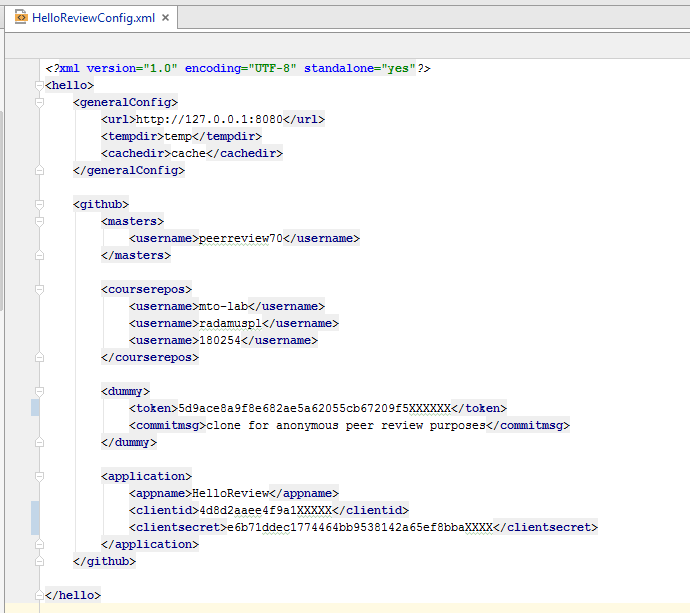
\includegraphics[width=400px]{0_3konfiguracja}
    \caption{Konfiguracja systemu - przykładowy plik}
    \label{obr03}
\end{figure}

\clearpage

Sekcja \textquote{generalConfig} zawiera zgrupowane ogólne luźno powiązane parametry ogólnego przeznaczenia:
\begin{itemize}
    \item url - adres URL do systemu, wykorzystywany jest on podczas autoryzacji przy użyciu protokołu OAuth2;
    \item tempdir - względna lub bezwzględna ścieżka do katalogu, który będzie wykorzystywany jako folder dla plików tymczasowych podczas anonimizacji prac;
    \item cachedir - względna lub bezwzględna ścieżka do katalogu, który będzie wykorzystywany jako pamięć podręczna podczas wykonywania połączeń do GitHub API.
\end{itemize}

\medskip
Sekcja \textquote{github} zawiera konfiguracje związane z~usługą GitHub.

Podsekcja \textquote{masters} zawiera listę nazw kont w~usłudze GitHub, należące do osób, które w~systemie posiadają uprawnienia prowadzących kurs.

Podsekcja \textquote{courserepos} zawiera listę nazw kont w~usłudze GitHub, które są wykorzystywane podczas kursów. Konta te wykorzystywane są jako źródło kursów. Na ich podstawie tworzona jest lista wyboru kursu podczas tworzenia nowego zlecenia przeglądu.

Podsekcja \textquote{dummy} zawiera token aplikacyjny usługi GitHub dla konta, które będzie wykorzystywane do anonimizacji prac. Na tym koncie przechowywane będą anonimowe kopie. Ponad to w~tej podsekcji ustawiony jest domyślny tekst dla akcji \textquote{commit} w~systemie kontroli wersji Git. Tekst ten zostanie użyty podczas procesu anonimizacji prac.

Podsekcja \textquote{application} definiuje dane autoryzujące aplikację w~usłudze GitHub.

\medskip
Znaczenie parametrów konfiguracji zostanie ściślej określone w~kolejnych rozdziałach, przy okazji opisu miejsc, gdzie są one wykorzystane.

\clearpage
\section{Rejestracja aplikacji w~usłudze GitHub}
Z uwagi na dużą skalę integracji z~usługą GitHub istotna część konfiguracji systemu jest związania właśnie z~tym serwisem. Autor zaleca rejestrację specjalnego konta przeznaczonego do użycia wyłączenie dla celów systemu. Jest to głównie związane z~tym, że składowane na nim będą anonimowe kopie ocenianych prac. Łatwo policzyć, że jeżeli na kurs chodzi 20 uczestników i~w danym momencie zarejestrujemy tylko jeden przegląd, gdzie każdy będzie musiał ocenić tylko jedną pracę to już jest 20 repozytoriów, które nie wyglądają profesjonalnie na koncie, i~odwracają uwagę od wartościowej zawartości. Ich ilość może być na tyle przytłaczająca, że inne treści zostaną zupełnie niezauważone.

\medskip
Rysunek nr \ref{obr04} zawiera zrzut ekranowy z~przykładem poprawnie zarejestrowanej aplikacji w~serwisie GitHub. Nazwę (\textquote{Application name}) i~opis (\textquote{Application description}) można dowolnie zmieniać. Istotne są natomiast adresy URL (\textquote{Homepage URL} i~\textquote{Authorization callback URL}). Ten pierwszy wskazuje na stronę domową, ten drugi natomiast musi wskazywać na podstronę \textquote{/callback}. To pod ten adres usługa GitHub przekieruje użytkownika po procesie logowania. Jest to jedyny poprawny adres, pod którym zostanie obsłużona informacja zwrotna.

\medskip
Ilustrowana strona zawiera także ciągi znaków \textquote{Client ID} i~\textquote{Client Secret}, które należy wprowadzić w~pliku konfiguracyjnym systemu. Istotne jest, aby ciąg \textquote{Client Secret} nie upubliczniać. Jest to ciąg związany z~mechanizmem autoryzacji \textquote{tożsamości} rejestrowanej aplikacji.

\begin{figure}[!h]
\centering
    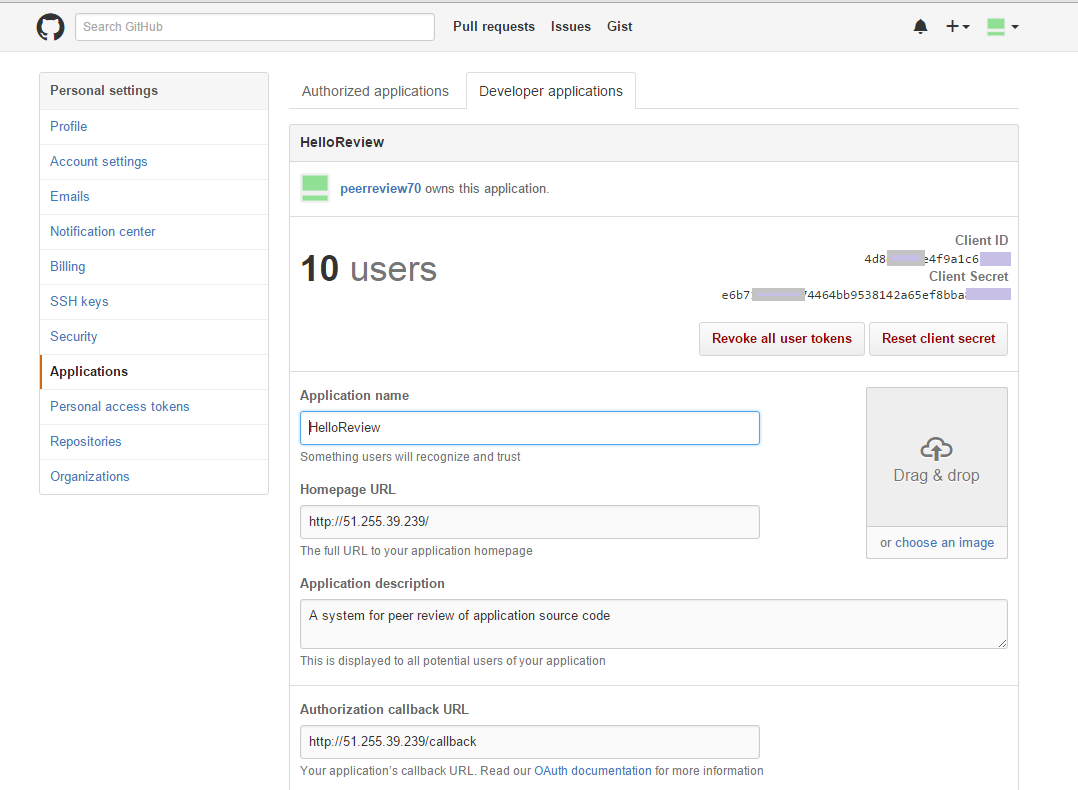
\includegraphics[width=340px]{0_4githubapp}
    \caption{Zrzut ekranowy: zarejestrowana aplikacja w~usłudze GitHub}
    \label{obr04}
\end{figure}

% ex: set tabstop=4 shiftwidth=4 softtabstop=4 noexpandtab fileformat=unix filetype=tex spelllang=pl,en spell:
    \chapter{Projekt i~implementacja systemu}

Autor nazwał system HelloReview (HR). Informacja ta ma charakter porządkowy, nazwa ta, lub jej skrót, występuje na załączonych rysunkach, może także wystąpić w~tekście.

Przepływ danych w~systemie wygląda następująco:

\begin{enumerate}
    \item Użytkownik loguje się do systemu następuje przy użyciu konta GitHub;
    \item Prowadzący zakłada kursy, do których zapisuje kursantów;
    \item Prowadzący tworzy projekt z~zadaniem na platformie GitHub;
    \item Kursant rozwiązując zadanie powielają odpowiedni projekt na platformie GitHub;
    \item Prowadzący zleca wzajemną ocenę postępów pracy dla danego projektu;
    \item Kursant ocenia pracę innego studenta wypełniając ankietę;
    \item Prowadzący sprawdza odpowiedzi w~systemie.
\end{enumerate}

Taki przebieg wydarzeń uwzględnia wszystkie wymagania w~stosunku do projektowanego systemu. W~rozdziale tym przedstawione zostaną szczegóły projektowe i~implementacyjne na bazie przedstawionych punktów. Przedstawienie projektu za zasadzie chronologicznie ułożonych wydarzeń ma na celu ułatwienie odbioru pracy, oraz zrozumienia budowy i~zasady działania systemu.

\newpage
\section{Logowanie do systemu}
Niezalogowany użytkownik po uruchomieniu strony internetowej nie posiada żadnych uprawnień. Zastaje on widok jak na zrzucie ekranowym na rysunku \ref{obr11}. Jedyną przewidzianą akcją w~tym momencie jest logowanie do systemu.

\begin{figure}[!h]
\centering
    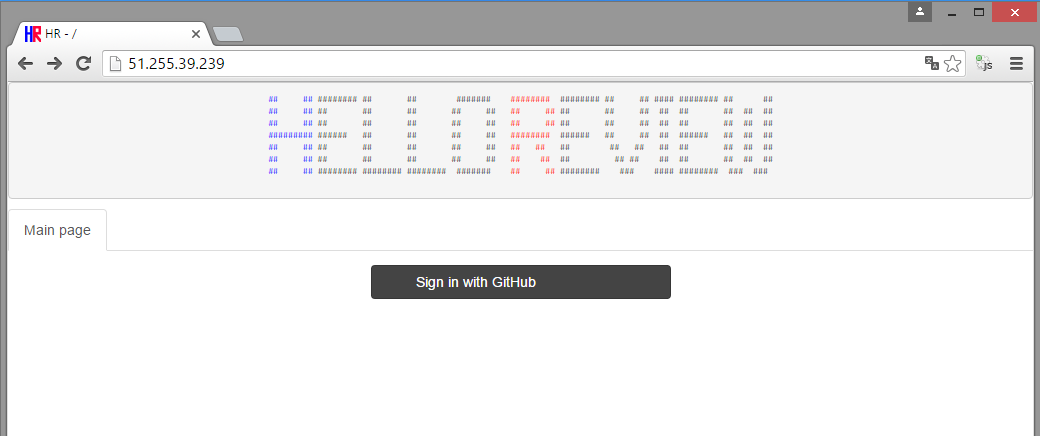
\includegraphics[width=\textwidth]{1_1logowanie}
    \caption{Zrzut ekranowy: strona główna dla niezalogowanego użytkownika}
    \label{obr11}
\end{figure}

Logowanie do systemu odbywa się przy użyciu usługi GitHub jako serwera autoryzacji. Autoryzacja następuje przy użyciu protokołu OAuth2. Użytkownik po kliknięciu w~przycisk zostaje przekierowany do platformy GitHub, gdzie potwierdza chęć udostępnienia danych systemowi, który go skierował. Wygląd potwierdzenia autoryzacji dla aplikacji przedstawia zrzut ekranowy na rysunku \ref{obr12}.

\begin{figure}[!h]
\centering
    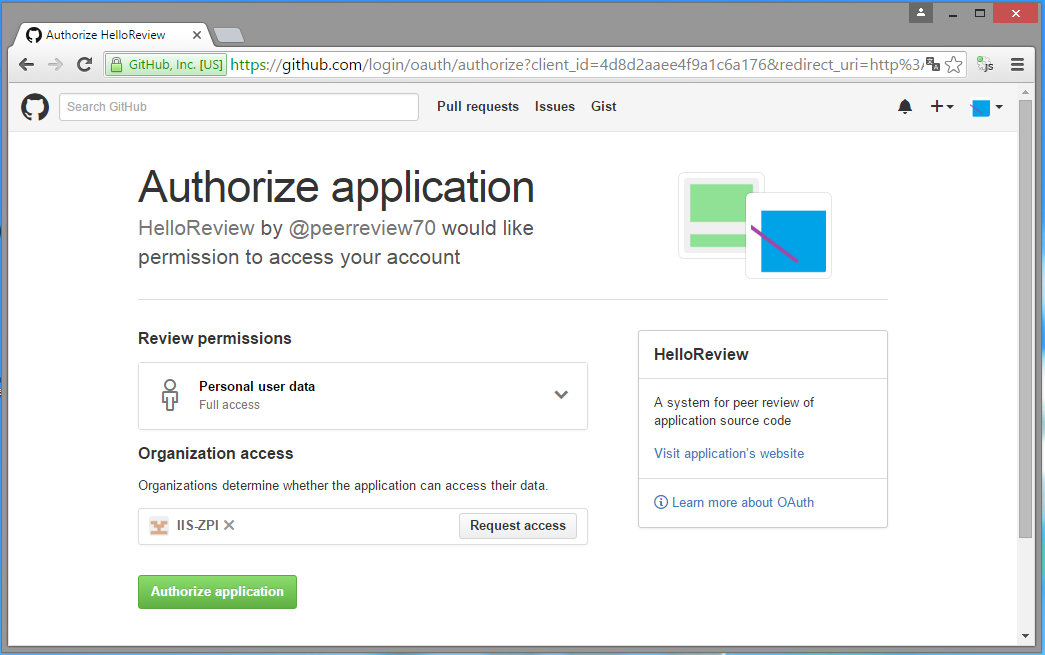
\includegraphics[width=375px]{1_2github}
    \caption{Zrzut ekranowy: autoryzacja aplikacji w~serwisie GitHub}
    \label{obr12}
\end{figure}

Jeżeli użytkownik potwierdził autoryzację system otrzymuje token autoryzacyjny, za pomocą którego może odczytać podstawowe dane na temat użytkownika. Najważniejszą informacją udostępnianą przez serwis GitHub jest nazwa użytkownika. To na jej podstawie system określa uprawnienia. Jeżeli nazwa zalogowanego użytkownika znajduje się w~pliku konfiguracyjnym, na liście w~sekcji \textquote{masters} to uzyskuje on dostęp z~prawami prowadzącego. W~przeciwnym razie ma on uprawnienia kursanta. Użytkownik, który nie zgodził się na udostępnienie danych nie może korzystać z~systemu. Wyrażenie braku zgody polega na zamknięciu zakładki z~akcją potwierdzenia, a~więc przerwaniu procesu potwierdzenia i~opuszczeniu systemu.

\medskip
Charakter systemu powoduje, że nie ma tu stopniowania uprawnień. Uprawnienia są rozłączone, co ułatwiło implementację kontroli uprawnień. Wszystkie podstrony pasujące do wzorca \textquote{/m/**} są przeznaczone dla prowadzącego, wzorzec \textquote{/p/**} odpowiada podstronom dedykowanym kursantom. Inne zasoby są ogólnodostępne, ich zawartość może być pobrana przez każdego - są to pliki statyczne, strona główna, oraz strony błędów.

\medskip
Kontrola uprawnień została zaimplementowana wykorzystując mechanizm \textquote{przechwytywania} (ang. intercept) żądań. Przed przejściem do właściwego kontrolera Spring uruchamia zdefiniowane mechanizmy wykonujące autoryzację. Rysunek numer \ref{kodi1} na stronie \pageref{kodi1} zawiera listing kodu z~klasą \textquote{InterceptorRegistryConfig}. Odpowiada ona za zarejestrowanie klas typu \textquote{interceptor}. Dwie z~zarejestrowanych klas są odpowiedzialne za kontrolę uprawnień. \textquote{InterceptorHasRoleMaster} sprawdza uprawnienia do podstron dla prowadzącego, oraz odpowiednio \textquote{InterceptorHasRoleMaster} sprawdza uprawnienia dla podstron dla kursantów.

\medskip
Rysunek numer \ref{kodi2} na stronie \pageref{kodi2} zawiera listing kodu z~klasą \textquote{InterceptorHasRoleMaster}. Autoryzacja polega na odpytaniu biblioteki pac4j, czy aktualnie użytkownik jest zalogowany, oraz sprawdzenie, czy jego nazwa użytkownika widnieje w~konfiguracji jako poprawna nazwa konta prowadzącego. Do komunikacji z~biblioteką pac4j autor napisał dodatkowo klasę użytkową \textquote{GHPac4jSecurityHelper}, która eksponuje jedynie rzeczy istotne dla systemu. Jeżeli użytkownik jest niezalogowany zostaje przekierowany do strony głównej. W~przypadku wykrycia próby uzyskania dostępu do zasobów przez zalogowanego użytkownika, do których nie ma uprawnień wysyłana jest odpowiedź ze stroną błędu o~kodzie \textquote{401 Unauthorized}. Autoryzacja uprawnień do podstron dla kursanta wygląda w~sposób odpowiadający - za kursanta system uważa każdego, kto nie został rozpoznany jako prowadzący.

\begin{figure}[!h]
\centering
    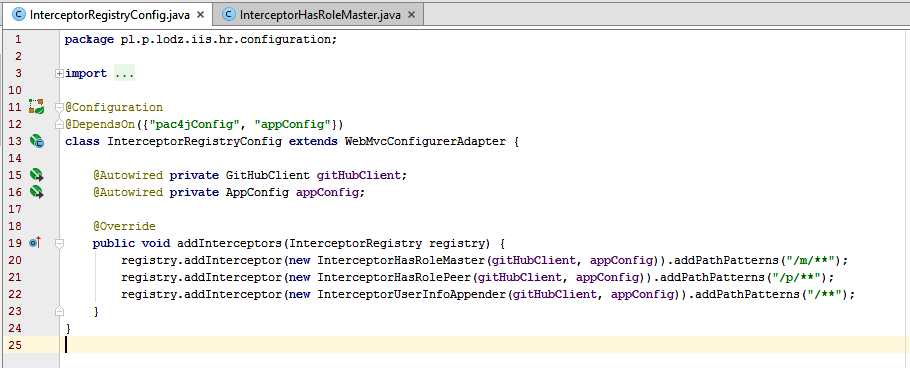
\includegraphics[width=\textwidth]{kod_interceptor1}
    \caption{Listing kodu źródłowego: klasa InterceptorRegistryConfig}
    \label{kodi1}
\end{figure}

\begin{figure}[!h]
\centering
    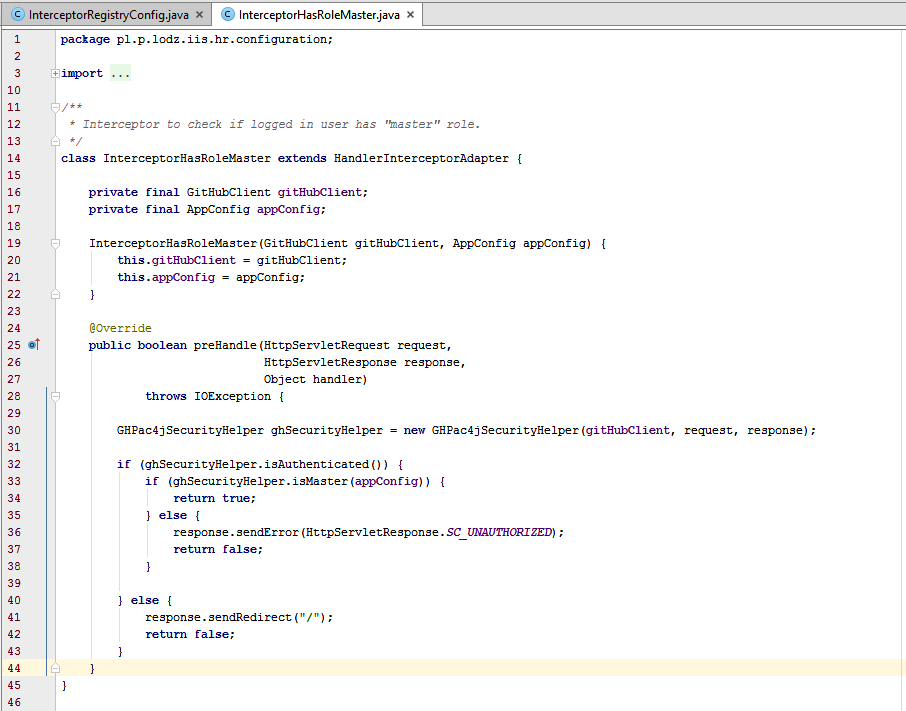
\includegraphics[width=\textwidth]{kod_interceptor2}
    \caption{Listing kodu źródłowego: klasa InterceptorHasRoleMaster}
    \label{kodi2}
\end{figure}

\clearpage
\section{Kursy i~ich uczestnicy}
Korzystanie z~systemu należy rozpocząć od zarejestrowania kursu i~przypisania do nich uczestników. System został tak zorganizowany, że na każdej podstronie widnieje lista znajdujących się zasobów danego typu (w~postaci tabelarycznej), a~pod nią przycisk dodania kolejnego. Obrazki \ref{obr21}, \ref{obr22}, \ref{obr23} zawierają kolejno zrzuty ekranowe przedstawiające: przykładową listę kursów, przykładową listę kursantów, i~przykład próby dodania kursu zakończonego niepowodzeniem, z~powodu niepowodzenia walidacji wprowadzonych danych.

\medskip
Kurs identyfikuje jedynie jego nazwa (ang. course name). W~przypadku kursanta należy podać dwie wartości: personalia (zwykle imię i~nazwisko) (ang. participant name) i~nazwę konta w~systemie GitHub (ang. GitHub nick, GitHub name). Poszukiwanie informacji dla danego kursanta, gdy ten się zaloguje do systemu, polega na porównaniu nazwy konta, z~którego się zalogował z~istniejącymi wpisami na temat uczestników w~bazie danych. Jest to jedyny warunek kontroli uprawnień do zasobów kursanta. Tożsamość została już wcześniej potwierdzona i~powiązana z~nazwą konta. Na tym etapie jest to warunek konieczny i~zupełnie wystarczający.

\medskip
\begin{figure}[!h]
\centering
    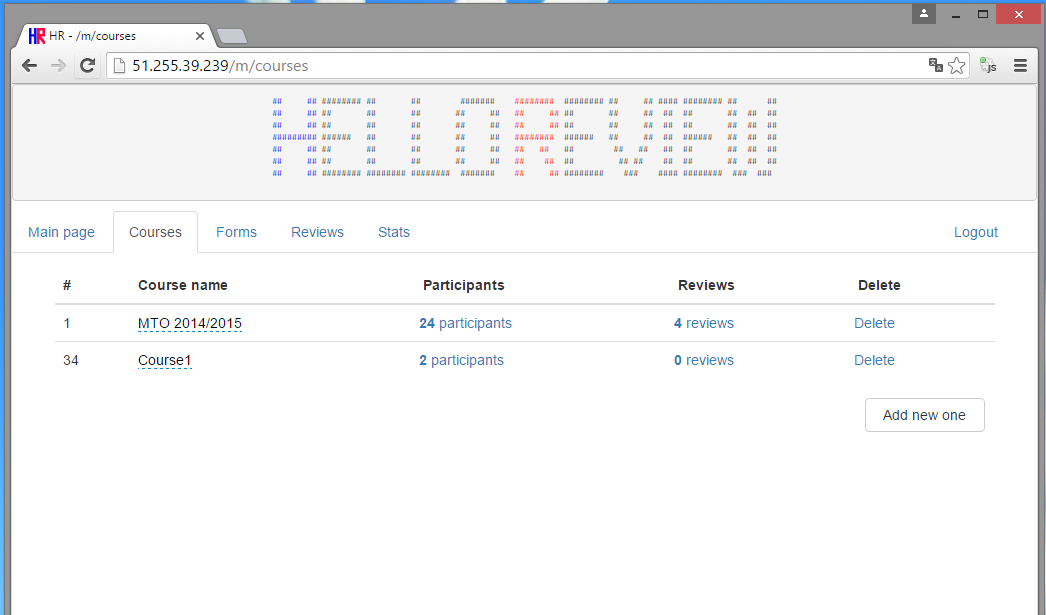
\includegraphics[width=\textwidth]{2_1kursy}
    \caption{Zrzut ekranowy: lista kursów}
    \label{obr21}
\end{figure}

\begin{figure}[!h]
\centering
    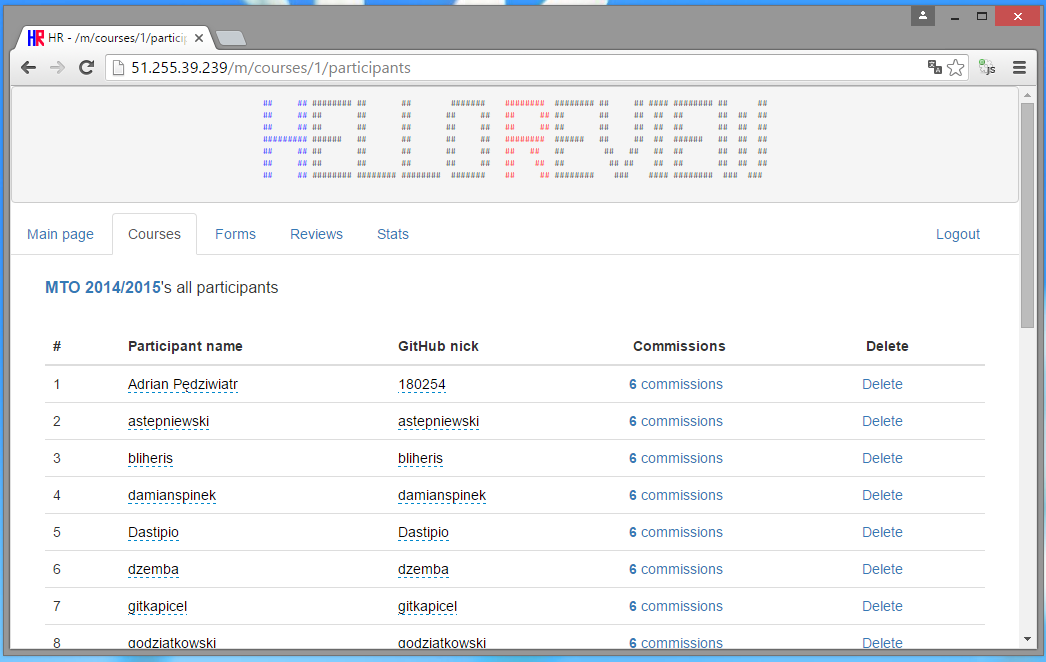
\includegraphics[width=\textwidth]{2_2kursanci}
    \caption{Zrzut ekranowy: lista kursantów}
    \label{obr22}
\end{figure}

\begin{figure}[!h]
\centering
    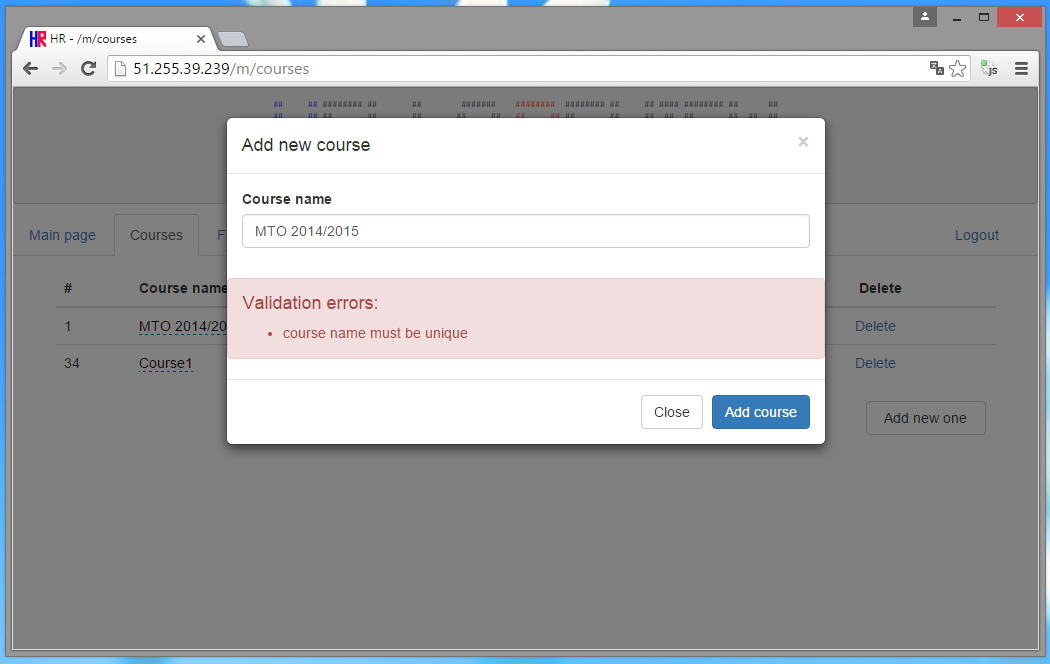
\includegraphics[width=\textwidth]{2_3dodanie}
    \caption{Zrzut ekranowy: formularz dodania kursu}
    \label{obr23}
\end{figure}

\clearpage
\section{Prowadzący umieszcza zadanie na platformie GitHub}
Prowadzący umieszcza dla każdego zadania nowe repozytorium Git na platformie GitHub. Przy czym nie chodzi tutaj o~umieszczenie w~nim samej treści zadania, a~o~projekt zawierający kod startowy. Założenie było wzorowane na laboratoriach, gdzie taki projekt bazowy zawierał kod, który należało rozbudować, poprawić lub uzupełnić o~przypadki testowe. Nic nie stoi na przeszkodzie jednak, by repozytorium takie było podstawowym ogólnym szablonem i/lub zawierało treść polecenia. Istotne jest jednak, że dla każdego zadania należy utworzyć oddzielne repozytorium.

\medskip
Założeniem jest jedno repozytorium = jeden przegląd, jedna ocena. Zgrupowanie zadań powoduje więc jednocześnie, że możliwość zlecenia przeglądu także istnieć będzie jedynie grupowo. Istnieje możliwość sprostowania, np. poprzez napisanie komentarza do zlecenia przeglądu, lecz użytkownik dostanie kopię całego repozytorium. Próba grupowania wydaje się więc być zbędną kombinacją, mimo wszystko możliwą jednak do realizacji.

\medskip
Dla systemu nie są istotne nazwy repozytoriów. Przykładową konwencją może być np. \textquote{lab\textunderscore X-Y}, gdzie X to kolejny numer zajęć, natomiast Y to numer zadania w~ramach danych zajęć.

\clearpage
\section{Kursant powiela repozytorium z~zadaniem}
Kursant rozwiązanie zadania rozpoczyna od powielenia (ang. fork) repozytorium na platformie GitHub. W~ten sposób system rozpoznaje, że kursant rozpoczął proces wykonania zadania, i~znajduje jego rozwiązanie. Z~uwagi na specyfikę dostępu do zasobów przy użyciu GitHub API istotne jest, aby kursant powielił projekt źródłowy. Błędem jest wielokrotne powielenie. Wielokrotne powielenie należy rozumieć jako powielenie repozytorium z~konta \textquote{X}, które jest powieleniem ze źródłowego konta \textquote{Y}. Należy mieć na uwadze opisane ograniczenie i~poinformować o~nim kursantów. Nieprawidłowe powielenie skutkować będzie nie wykryciem rozwiązania kursanta przez system, co może budzić różne konsekwencje, w~zależności od woli prowadzącego kurs. Rysunek numer \ref{obr41} zawiera zrzut ekranowy z~platformy GitHub, na którym widać, iż projekt został wielokrotnie powielony, lecz kursant o~nazwie konta \textquote{grzego699} wykonał to nieprawidłowo (w~rozumieniu ograniczeń systemu).

\begin{figure}[!h]
\centering
    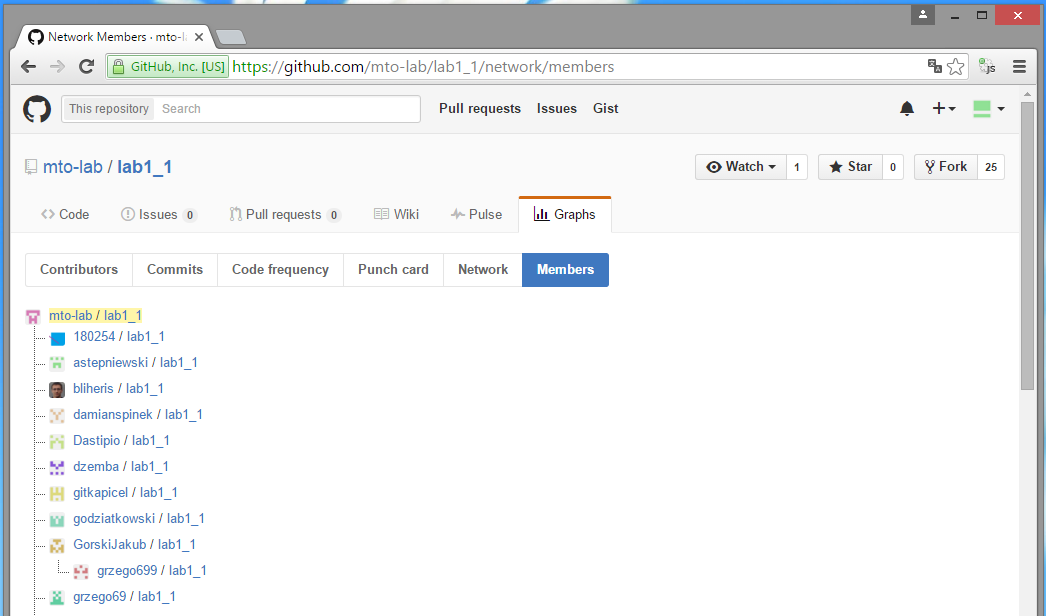
\includegraphics[width=\textwidth]{4_1forks}
    \caption{Zrzut ekranowy: powielenia repozytorium na platformie GitHub}
    \label{obr41}
\end{figure}

\clearpage
\section{Prowadzący zleca przegląd}

\subsection{Formularz oceny}
Jedną ze składowych przeglądu jest formularz, za pomocą którego będzie dokonana ocena. Przed przejściem do właściwej części zlecenia przeglądu należy zastanowić się, czy zastosowanie ma jakiś z~istniejących już w~systemie formularzy, czy też należy dodać następny. 

\medskip
W skład formularza wchodzą następujące składowe:
\begin{itemize}
    \item opis (ang. description) - ogólny informacja dla studenta na temat zadania, które ma aktualnie wykonać (przegląd i~ocena). Opis powinien zawierać dwa znaczniki specjalne \{project\} i~\{url\}. Pierwszy z~nich zostanie w~ostatecznej wersji zastąpiony nazwą projektu (tj. repozytorium), którego ocena następuje. Drugi natomiast zostanie zamieniony na adres do anonimowej kopii, gdzie kursant może się zapoznać z~ocenianą pracą;
    \item pytania (ang. questions) - lista pytań, na które kursant musi odpowiedzieć.
\end{itemize}

\medskip
Pytanie w~formularzu składa się z~następujących składowych:
\begin{itemize}
    \item tekst pytania (ang. question text) - treść pytania;
    \item dodatkowe wskazówki (ang. additional tips) - dodatkowa treść umieszczana zaraz pod treścią główną pytania. Jej przeznaczeniem jest przekazanie kursantowi dodatkowych wskazówek (np. na co powinien zwrócić szczególną uwagę), czy też dowolna inna treść uzupełniająca pytanie. Element ten nie jest obowiązkowy i~nie musi być w~pytaniu wykorzystywany;
    \item kontrolki (ang. inputs) - pola, które służą do wprowadzenia odpowiedzi na pytanie przed kursanta. System obecnie obsługuje dwa rodzaje kontrolek. Kontrolka typu tekst (ang. text) pozwala na wprowadzenie dowolnej treści tekstowej do 10 000 znaków. Kontrolka typu skala (ang. scale) pozwala wyrazić ocenę w~skali liczbowej. Zakres skali, oraz jej znaczenie semantyczne jest bez znaczenia w~sensie technicznym. Pytanie może składać się z~wielu kontrolek - brak jest ograniczeń w~tym względzie. Podczas generowania formularza ich kolejność zostanie zachowana. Kontrolka może zostać oznaczona jako obowiązkowa do wypełnienia lub nie. Z~powodu ograniczeń technicznych systemu parametr ten ma zastosowanie tylko dla kontrolki typu tekst. Wypełnienie kontrolki typu skala zawsze jest obowiązkowe.
\end{itemize}

\clearpage
\medskip
Formularz do systemu wprowadza się poprzez plik XML o~odpowiedniej strukturze. Struktura ta jest sprawdzana pod kątem obecności wszystkich obowiązkowych składowych i~poprawności składniowej. System pozwala na wyświetlenie struktury XML już zdefiniowanych formularzy. Możliwy jest także podgląd wyglądu formularza po jego wygenerowaniu. Wyświetlony formularz jest identyczny z~tym, który zostanie wyświetlony kursantowi. Rysunki o~numerach \ref{obr511}-\ref{obr513} zawierają zrzuty ekranowe z~procesu dodawania formularza do systemu.

\medskip
Plik XML podany przez użytkownika jest przetwarzany na klasę \textquote{Form}, będąca jednocześnie encją. Za tą formę \textquote{deserializacji} odpowiada biblioteka \textquote{Jackson}. Następnie system sprawdza, czy przekazany formularz jest prawidłowy. Kontrola ta polega na upewnieniu się, że wszystkie wymagane pola zostały uzupełnione i~nie są puste. Za proces walidacji odpowiada zastosowana biblioteka \textquote{Hibernate}, a~dokładnie moduł który nazywa się \textquote{Hibernate Validator}. W~przypadku niepowodzenia walidacji prowadzący otrzymuje odpowiednie szczegóły, niezbędne do jego poprawienia. Jeżeli kod formularza okazał się być prawidłowy encja zostaje zapisana w~bazie danych i~podgląd formularza może zostać wyświetlony użytkownikowi.

\begin{figure}[!h]
\centering
    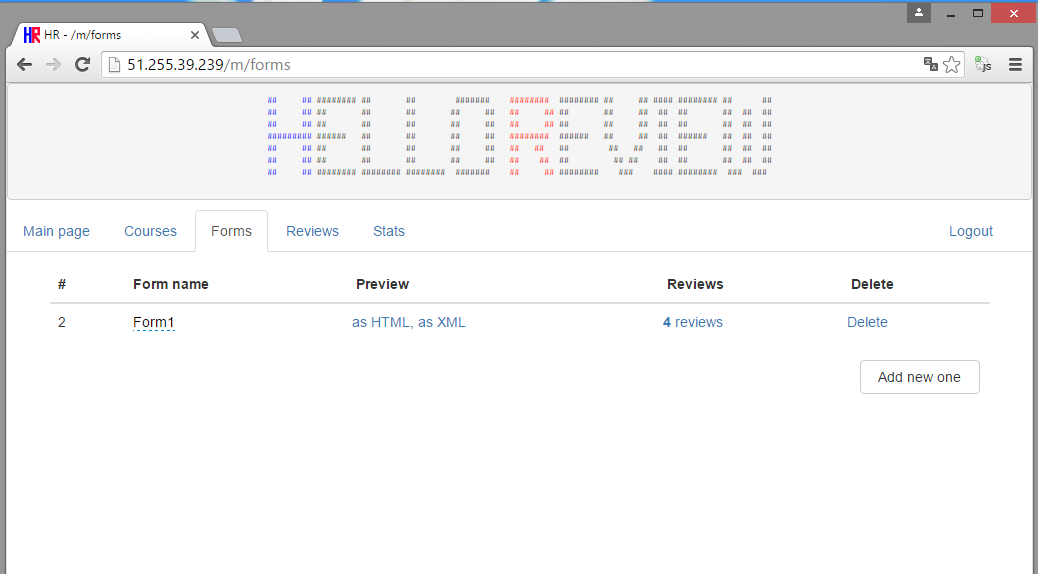
\includegraphics[width=\textwidth]{5_1_1formlist}
    \caption{Zrzut ekranowy: lista formularzy w~systemie}
    \label{obr511}
\end{figure}


\begin{figure}[!h]
\centering
    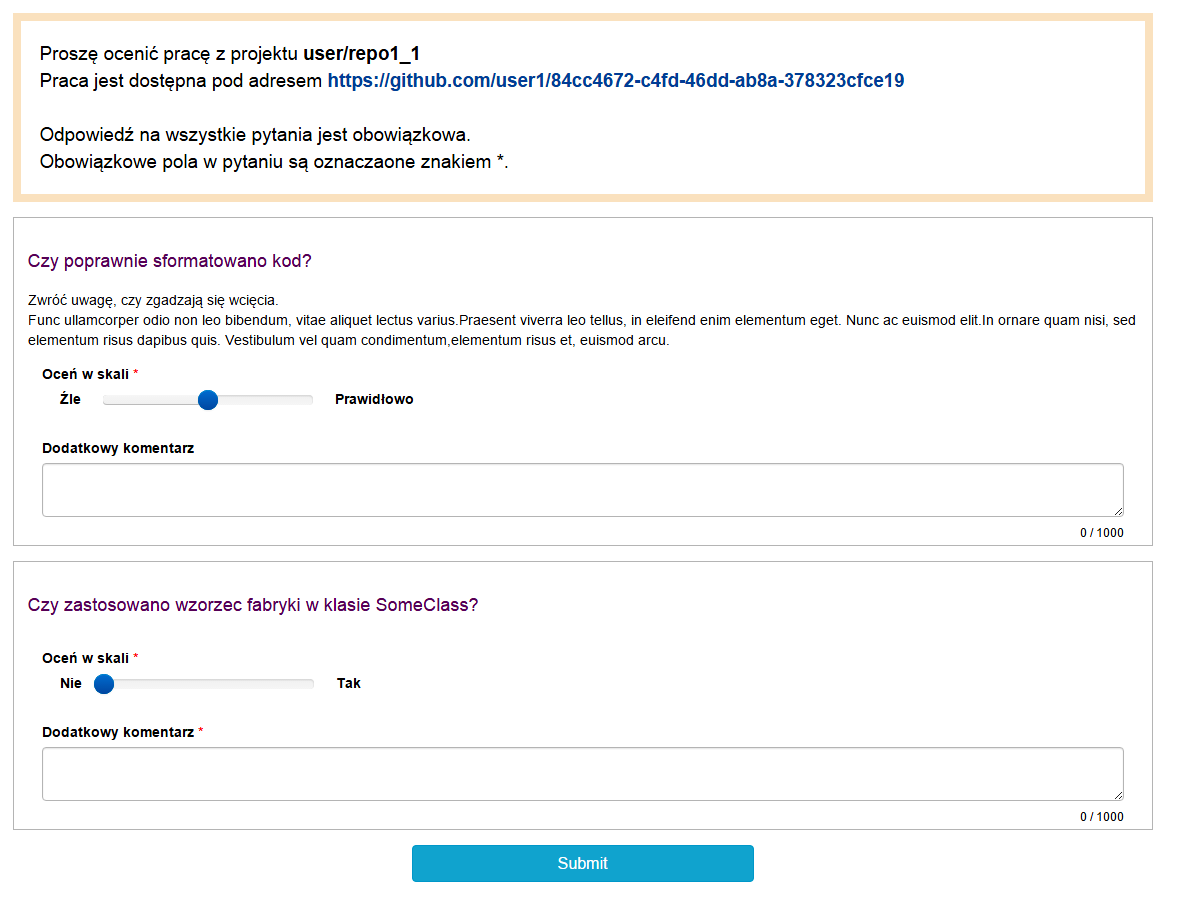
\includegraphics[width=\textwidth]{5_1_2poglad}
    \caption{Zrzut ekranowy: podgląd formularza po jego wygenerowaniu}
    \label{obr512}
\end{figure}


\begin{figure}[!h]
\centering
    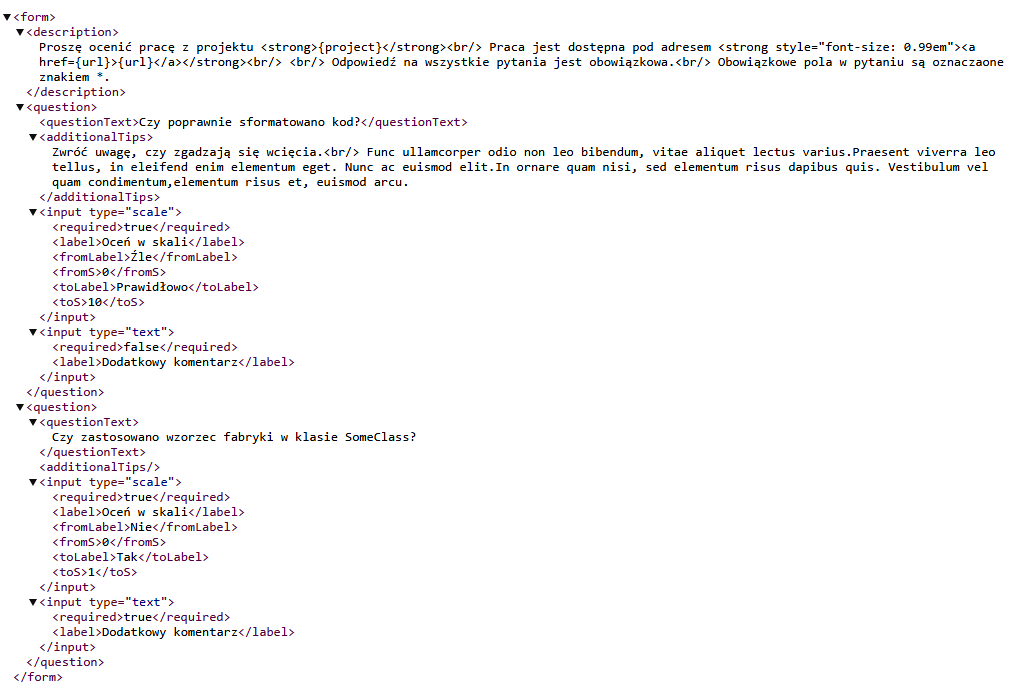
\includegraphics[width=\textwidth]{5_1_3xml}
    \caption{Zrzut ekranowy: przykładowy plik XML z~definicją formularza}
    \label{obr513}
\end{figure}

\clearpage
\subsection{Zlecenie przeglądu}
Rysunek numer \ref{obr521} zawiera zrzut ekranowy z~listą przeglądów w~systemie. Lista jest przedstawiona w~sposób tabelaryczny i~zawiera następujące informacje:
\begin{itemize}
    \item nazwa przeglądu (ang. review name);
    \item odnośnik do kursu (ang. course) związanego z~przeglądem;
    \item odnośnik do formularza (ang. form) związanego z~przeglądem;
    \item odnośnik ocenianego projektu (repozytorium; ang. repository) związanego z~przeglądem;
    \item liczba zleceń oceny na osobę (ang. commissions per peer);
    \item odnośnik do statusu zleceń (ang. commissions);
    \item odnośnik do odpowiedzi (ang. responses);
    \item status zamknięcia (ang. close state).
\end{itemize}

\begin{figure}[!h]
    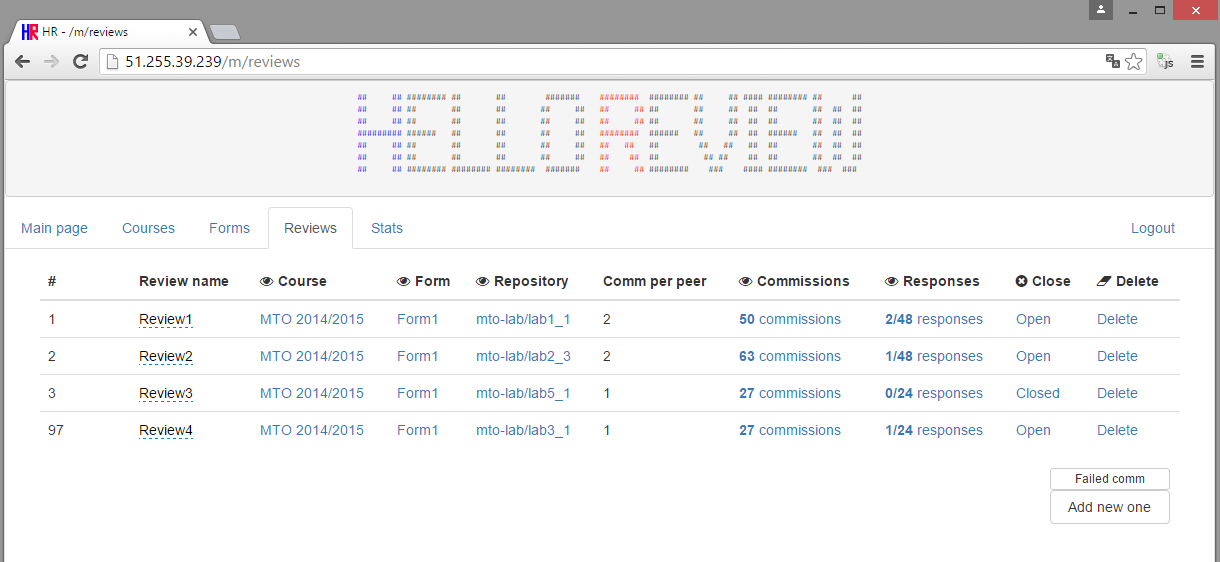
\includegraphics[width=\textwidth]{5_2_1rlista}
    \caption{Zrzut ekranowy: lista przeglądów w~systemie}
    \label{obr521}
\end{figure}

\medskip
Pod listą stworzonych już przeglądów, zgodnie z~zastosowaną konwencją, znajduje się przycisk do formularza, za pomocą którego możliwe jest dodanie nowego przeglądu. Wygląd formularza przedstawia zrzut ekranowy na rysunku \ref{obr523}.

\medskip
Formularz dodawania przeglądu wymaga podania następujących informacji:
\begin{itemize}
    \item nazwa przeglądu (ang. review name) - unikatowa nazwa nowo tworzonego przeglądu;
    \item liczba zleceń na kursanta (ang. number of commissions per participant) - określa ile prac ma ocenić każdy z~kursantów. Przydział prac do oceniania jest losowy. Nie ma jednak możliwości, by kursant dostał dwa tą samą pracę do ocenienia. Nie ma też możliwości ręcznego dokonania przydziału; 
    \item kurs związany z~przeglądem (ang. course) - należy wskazać z~listy kurs, dla którego zostanie utworzony przegląd;
    \item formularz związany z~przeglądem (ang. form) - należy wskazać z~listy formularz, który zostanie użyty do oceny;
    \item repozytorium projektu związanego z~przeglądem (ang. repository) - należy wskazać repozytorium projektu, którego rozwiązania kursanci mają dokonać oceny. 
\end{itemize}

\medskip
Przegląd jest pojęciem ogólnym i~dotyczy zadania w~ramach grupy - prowadzący zlecił dokonanie przeglądu danego zadania, w~danej grupie. Przegląd składa się ze zleceń. Zlecenie jest to pojedyncze zadanie ocenienia pracy autorstwa~A przez osobę~B.

\medskip
Po potwierdzeniu chęci wykonania przeglądu poprzez przycisk \textquote{stwórz przegląd} (ang. create review) system dokona sprawdzenia, czy wszyscy kursanci prawidłowo wykonali powielenie projektu. Policzy także efektywną liczbę zleceń na kursanta. Jeżeli podana w~formularzu liczba nie jest możliwa do osiągnięcia, zostanie ona obniżona do najbliższej możliwej wartości. Zrzut ekranowy na rysunku \ref{obr523} przedstawia widok z~wyświetlonymi informacjami wstępnymi. Jeżeli proces tworzenia przeglądu zostanie potwierdzony, system wykona tą czynność, a~następnie uruchomi algorytm anonimizacji prac.

\medskip
System umożliwia zamknięcie przeglądu. Zamknięcie przeglądu powoduje, że użytkownik nie będzie mógł już udzielić odpowiedzi. Anonimowe kopie związane z~przeglądem zostają oznaczone jako niepotrzebne, i~usunięte w~trakcie najbliższego procesu czyszczenia. 

\begin{figure}[!h]
    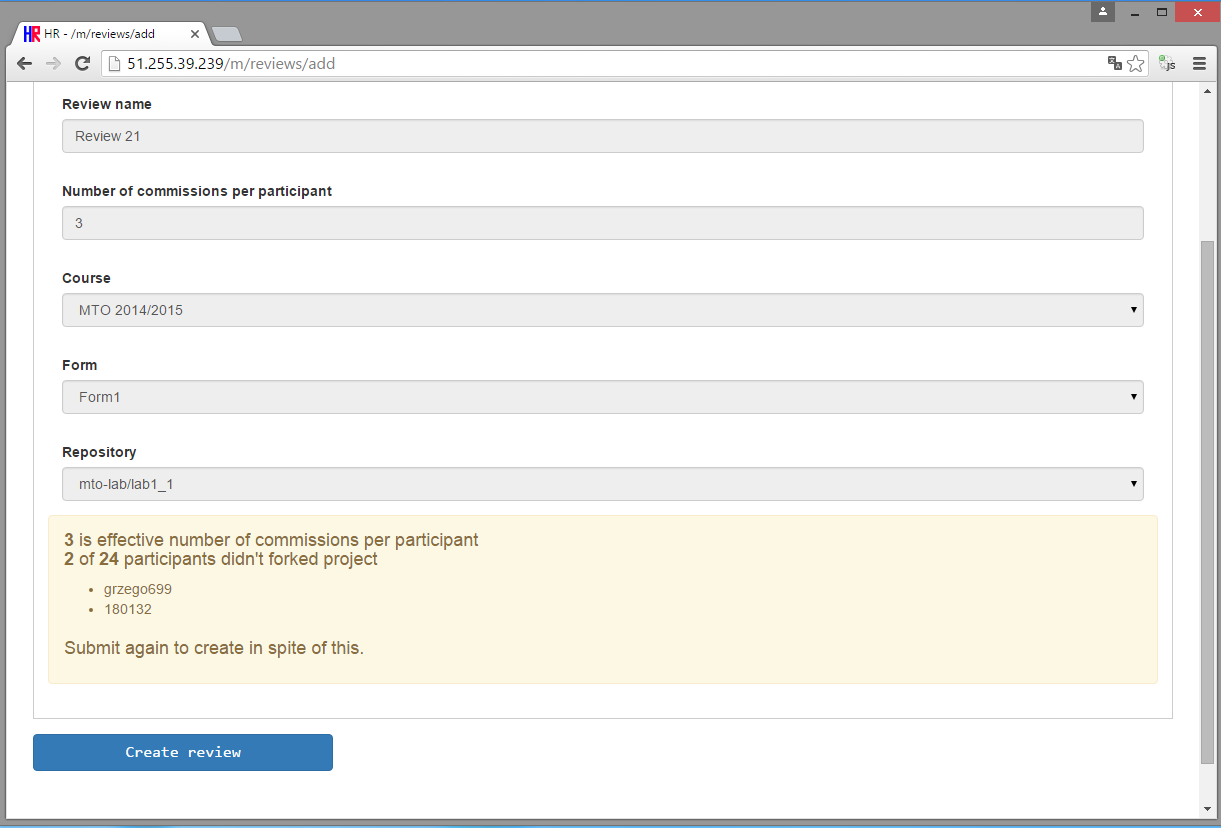
\includegraphics[width=405px]{5_2_3_radd2}
    \caption{Zrzut ekranowy: formularz dodawania przeglądu}
    \label{obr523}
\end{figure}

\clearpage
Rysunki numer \ref{kodp1} oraz \ref{kodp2} zawierają listing kodu źródłowego. Są to dwie części kodu z~klasy \textquote{GHReviewCreator}, która odpowiada za proces przygotowania przeglądu i~zarejestrowania wszystkich zleceń do wykonania. Pierwszy z~nich zawiera fragment do momentu sprawdzenia, ile osób nie wywiązało się z~zadania i~wyświetlenia tej informacji prowadzącemu, celem uzyskania potwierdzenia chęci kontynuacji. Po potwierdzeniu zastosowanie znajduje kod zamieszczony na drugim listingu. Funkcję, której listing zamieszczono wywołuje kontroler, odpowiedzialny za podstronę zlecania przeglądów. Przekazywany do niej zostaje wypełniony formularz (obiekt typu \textquote{GHReviewAddForm}), repozytorium z~zadaniem (obiekt typu \textquote{GHRepository)} oraz obiekt umożliwiający zmianę stanu wysyłanej odpowiedzi HTTP (\textquote{HttpServletResponse}). Funkcja zwraca numer nowo utworzonego przeglądu.

\begin{figure}[!h]
    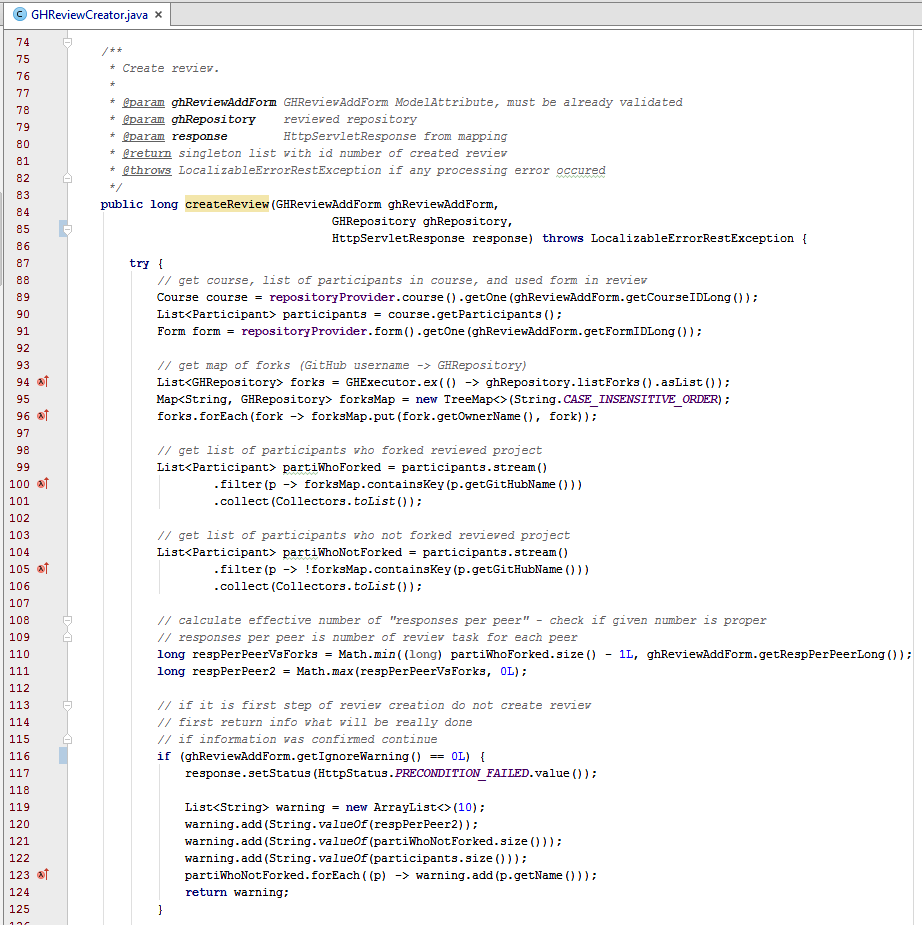
\includegraphics[width=\textwidth]{kod_przeglad}
    \caption{Listing kodu źródłowego: tworzenie przeglądu, klasa GHReviewCreator (część 1)}
    \label{kodp1}
\end{figure}

\begin{figure}[!h]
    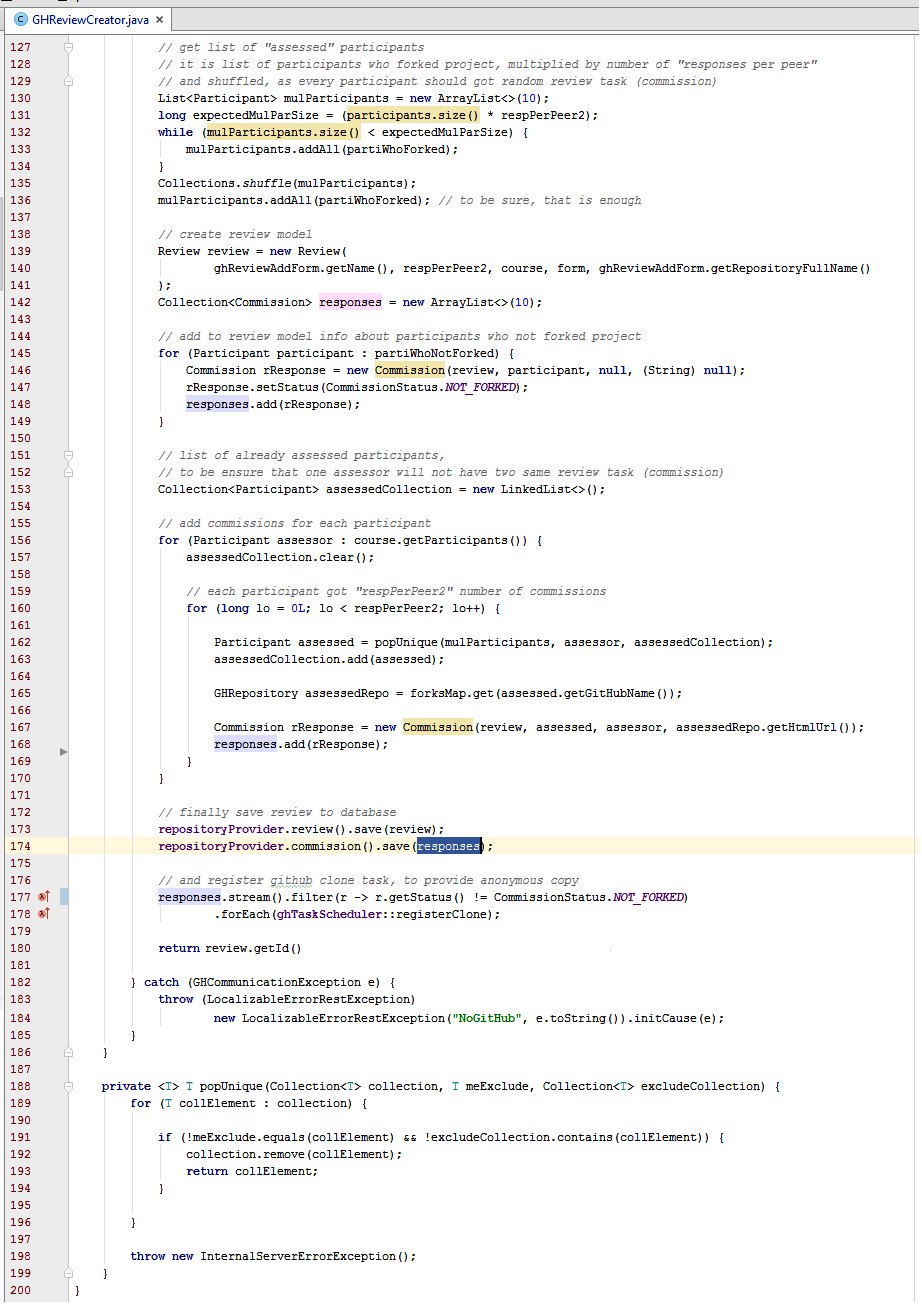
\includegraphics[width=\textwidth]{kod_przeglad2}
    \caption{Listing kodu źródłowego: tworzenie przeglądu, klasa GHReviewCreator (część 2)}
    \label{kodp2}
\end{figure}

\clearpage
\subsection{Algorytm anonimizacji prac}
Z momentem utworzenia przeglądu system uruchomił algorytm odpowiedzialny za anonimizację prac. W~tym momencie lista zleceń jest już znana, zostały ustalone adresy repozytoriów źródłowych - było to niezbędne już na wcześniejszym etapie. Dla każdego zlecenia system dokonuje kopiowania pracy. Za skopiowanie pracy jest odpowiedzialna klasa GHTaskClone. Proces kopiowania przebiega zgodnie ze schematem:

\begin{enumerate}
    \item system zgłasza zlecenie: Kursant1 ma ocenić pracę Kursant2;
    \item system nadaje zleceniu indywidualny unikalny ID, zgodny ze standardem UUID4;
    \item system zakłada repozytorium zdalne na koncie \textquote{manekin} (ang. dummy), którego token został podany w~pliku konfiguracyjnym, o~nazwie takiej, jak nadany ciąg ID;
    \item system sprawdza listę gałęzi (ang. branch) w~kopiowanym repozytorium;
    \item system kopiuje każdą ze znalezionych gałęzi:
    \begin{enumerate}
        \item system pobiera do folderu tymczasowego (zdefiniowanego znacznikiem \textquote{tempdir} w~pliku konfiguracyjnym) wybraną gałąź z~repozytorium źródłowego, na tym folderze wykonuje kolejne akcje;
        \item system usuwa ukryty folder \textquote{.git} - projekt przestaje być repozytorium Git;
        \item system inicjalizacje nowe puste repozytorium lokalne;
        \item system konfiguruje nowe repozytorium - nazwa użytkownika i~adres e-mail zostają ustawione na takie, które widnieją w~konfiguracji konta \textquote{dummy} na platformie GitHub;
        \item system zapisuje zmiany (w~tym przypadku: wszystkie istniejące pliki) w~repozytorium lokalnym (akcja git: commit), treścią używaną do opisu zmian jest ciąg \textquote{commitmsg} ustalony w~pliku konfiguracyjnym;
        \item system wysyła skopiowaną lokalnie gałąź do repozytorium zdalnego (git push);
    \end{enumerate}
    \item system sprawdza jaka gałąź w~repozytorium źródłowym jest ustawiona jako domyślna (ang. default), takiego samego ustawienia dokonuje na kopii;
    \item system zapisuje adres utworzonej kopii w~bazie danych - to ten adres zostanie przekazany recenzentowi.
\end{enumerate}

Jeżeli proces kopiowania nie powiedzie się, na jakimkolwiek etapie, zmiany są wycofywane. W~bazie danych zostaje zapisana odpowiednia informacja o~porażce. Niepowodzenie może być spowodowane wieloma czynnikami. Najprostszą przyczyną jest niedostępność jednej z~usług platformy GitHub. Inną możliwą przyczyną jest niedoskonałość implementacji algorytmu, który zawiódł z~bliżej nieokreślonej przyczyny - podczas testów przypadek taki został zanotowany dla około pół procent zleceń. Autor po konsultacji z~opiekunem pracy ustalił, że zbadana niezawodność jest wystarczająca. Proces ponowienia próby kopiowania nie jest dokonywany automatycznie, należy go uruchomić manualnie. System przewiduje odpowiednią opcję dostępną w~podglądzie stanów zleceń.

\medskip
\textquote{Esencję} algorytmu anonimizacji zawiera obrazek \ref{kodanon} na stronie \pageref{kodanon}. Jest to listing funkcji \textquote{run} z~klasy \textquote{GHTaskClone}. Wspominana klasa reprezentuje zadanie anonimizacji prac i~wykonuje kolejne czynności zgodnie z~zaprezentowanych schematem.

\medskip
Jak wspomniano, w~systemie istnieje możliwość podglądu stanów zleceń oceny w~ramach przeglądu. Podgląd ten został zaprezentowany na zrzucie ekranowym na obrazku numer \ref{obr524} na stronie \pageref{obr524}. Widniejący tam status może przyjąć następujące wartości:

\begin{itemize}
    \item projekt nie powielony (ang. project not forked) - informacja dodatkowa, wpis taki jest tworzony dla każdego kursanta, którego rozwiązanie nie zostało znalezione. W~sposób naturalny praca takiego kursanta nie może zostać oceniona. Sam kursant jednak oczywiście dostaje do oceny inne prace;
    \item przetwarzanie zakończone porażką (ang. processing failed) - proces kopiowania zakończył się niepowodzeniem. W~przypadku niepowodzenia obok zlecenia staje się dostępny przycisk pozwalający ponowić próbę (ang. retry) anonimizacji dla tej pracy;
    \item w~trakcie przetwarzania (ang. processing) - anonimizacja dla tego zlecenia została zaplanowana, lub jest w~trakcie przetwarzania. System kolejkuje zlecenia, wykonując jednocześnie nie więcej niż trzy kopie.
    \item ocena nie wypełniona (ang. unfilled) - proces anonimizacji zakończył się powodzeniem i~formularz oceny jest dostępny dla kursanta. Kursant nie dokonał jeszcze oceny;
    \item ocena wypełniona (ang. filled) - kursant dokonał oceny.
\end{itemize}

\medskip
Jak już zostało wyjaśnione kopie są składowane na specjalnie do tego przeznaczonym koncie. Obrazek \ref{526schemat} przedstawia schematycznie obieg repozytorium. Zrzut ekranowy na obrazku \ref{obr525} na stronie \pageref{obr525} przedstawia natomiast przykładową listę repozytoriów widoczną na takim koncie.

\begin{figure}[!h]
    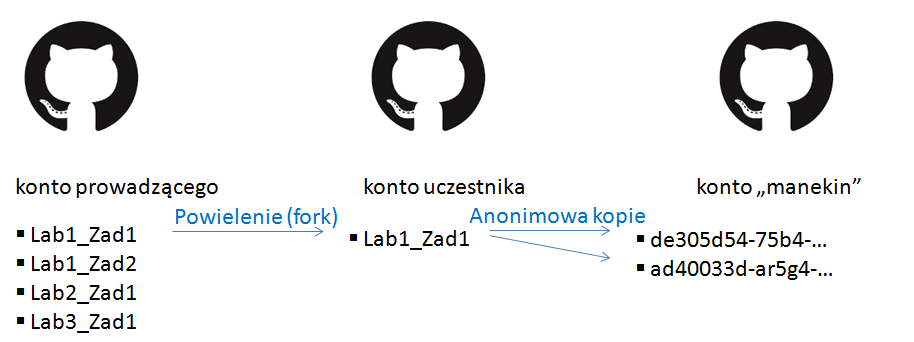
\includegraphics[width=290px]{5_2_6schemat}
    \caption{Repozytorium z zadaniem i jego powielenia nad kontach w usłudze GitHub}
    \label{526schemat}
\end{figure}

\begin{figure}[!h]
    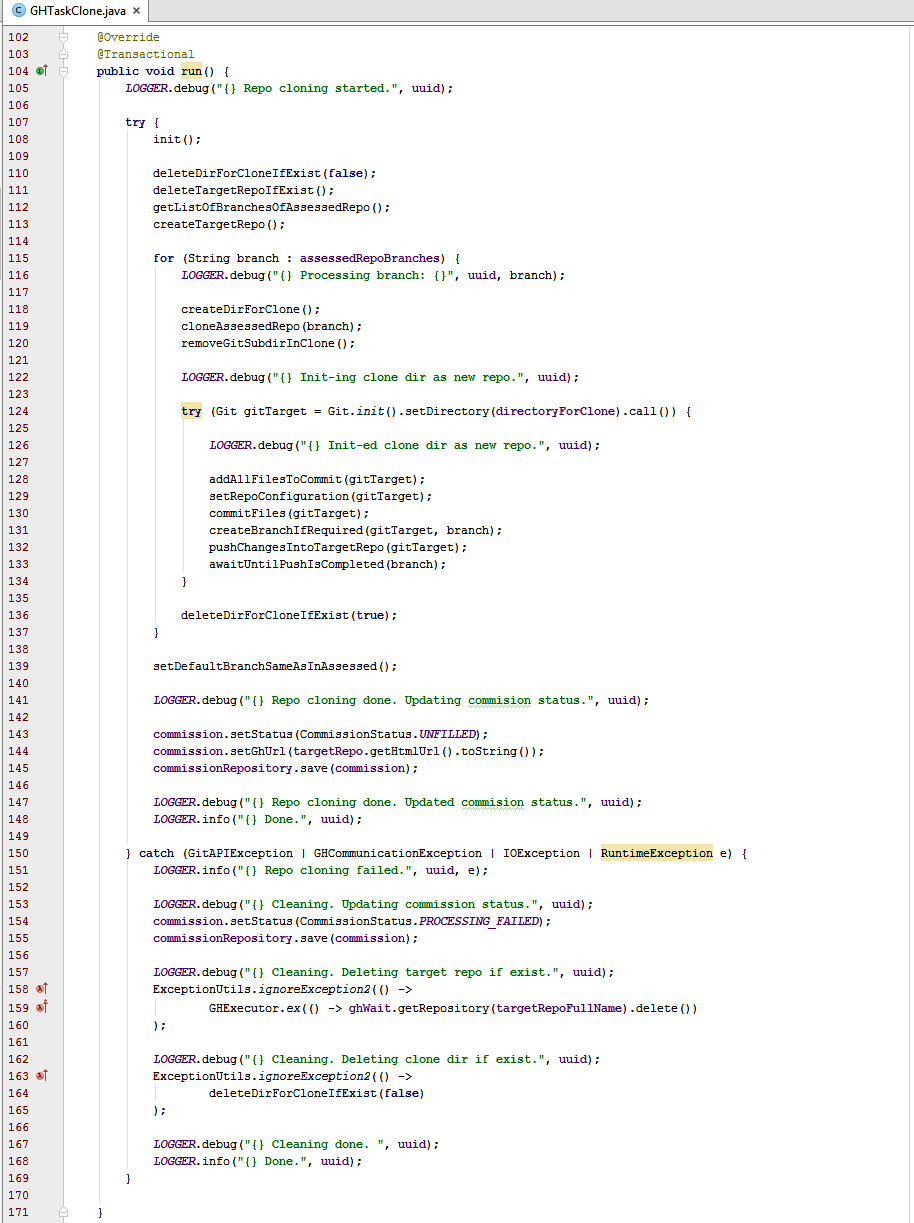
\includegraphics[width=\textwidth]{kod_klonowanie}
    \caption{Listing kodu źródłowego: anonimizacja prac, kopiowanie repozytorium}
    \label{kodanon}
\end{figure}


\begin{figure}[!h]
    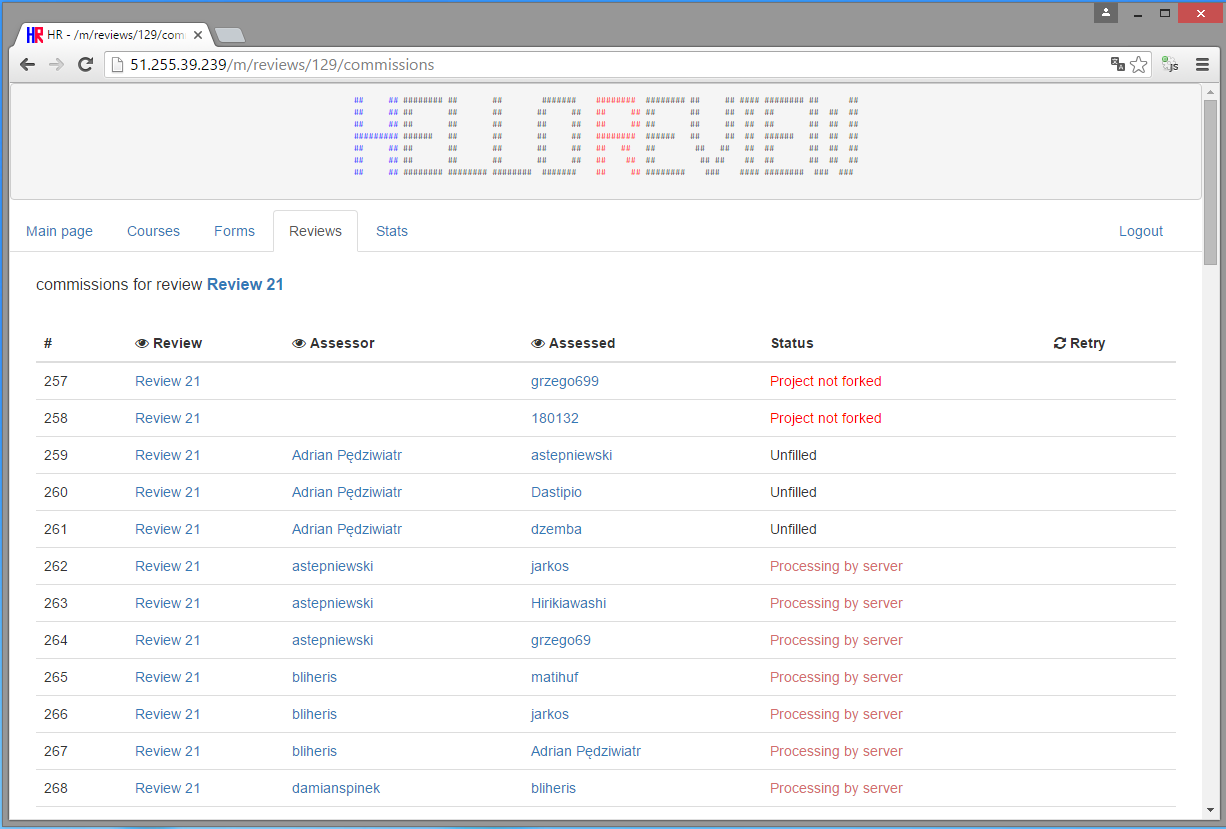
\includegraphics[width=\textwidth]{5_2_4status}
    \caption{Zrzut ekranowy: status zleceń w~przeglądzie}
    \label{obr524}
\end{figure}

\begin{figure}[!h]
    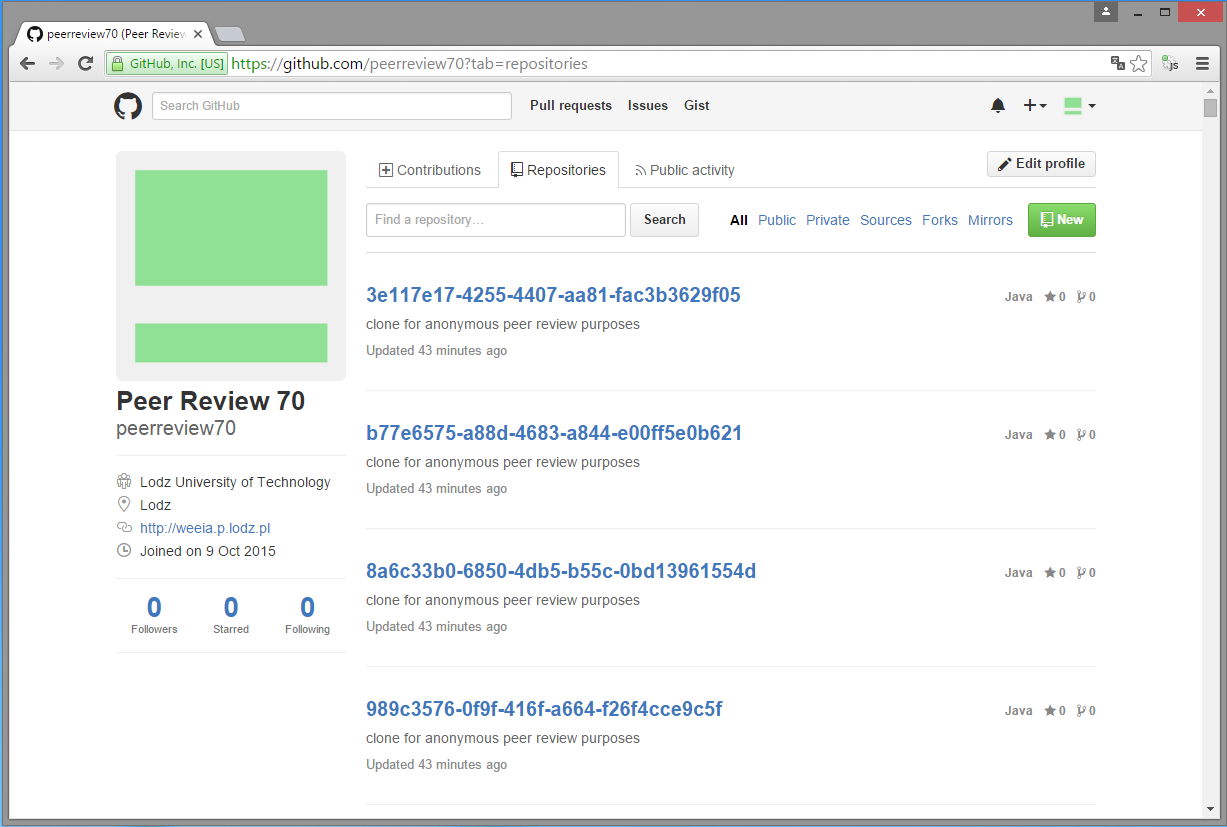
\includegraphics[width=\textwidth]{5_2_5dummyrepo}
    \caption{Zrzut ekranowy: anonimowe kopie zleceń w~usłudze GitHub}
    \label{obr525}
\end{figure}

\clearpage
\section{Kursant dokonuje oceny}
Kursant po zalogowaniu do systemu widzi listę zleceń. Rysunek ze zrzutem ekranowym numer \ref{obr61} przedstawia przykładową listę. Jeżeli zlecenie zostało już poprawnie przetworzone przez algorytm anonimizujący, przegląd nie jest zamknięty a~odpowiedź jeszcze nie udzielona użytkownik może wykonać przydzielone mu zadanie - dokonać przeglądu i~oceny pracy. Zlecenia takie zostały wyróżnione na liście szarym kolorem, oraz czerwoną lewą i~prawą krawędzią tabeli. Adres do formularza oceny znajduje się jako ostatnia pozycja na liście. Adres do formularza, sam formularz, ani żadna inna informacja nie ujawnia autora ocenianego rozwiązania. Kursant zna tylko indywidualny numer zlecenia, który nie zdradza tej informacji, ani nie daje się z niczym powiązać (między innymi z uwagi na zastosowaną losowość ID).

\begin{figure}[!h]
    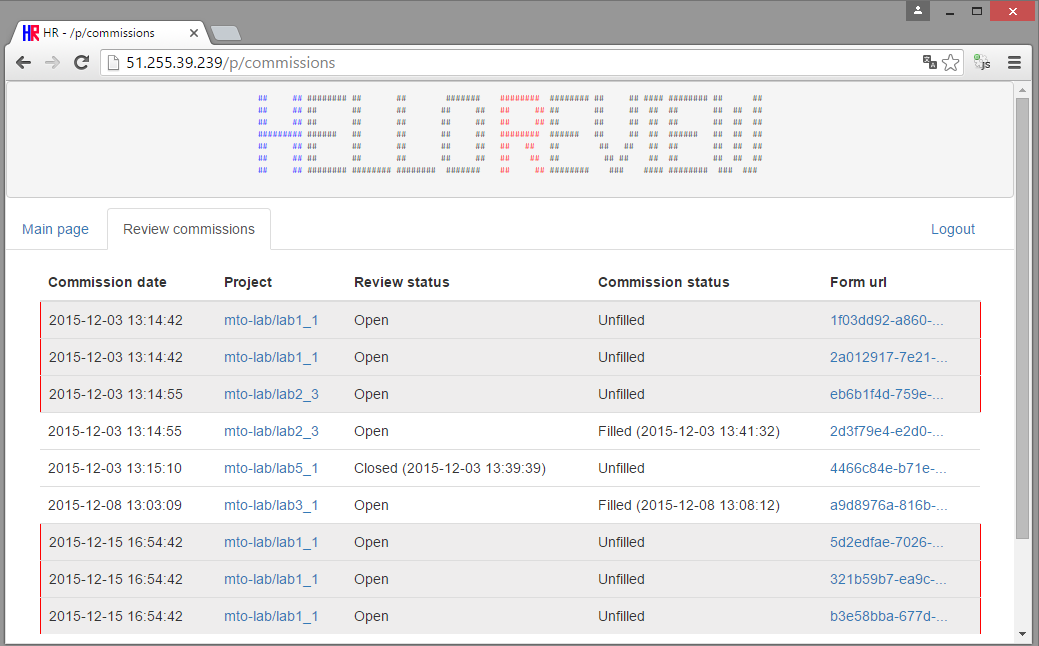
\includegraphics[width=\textwidth]{6_1zlecenia}
    \caption{Zrzut ekranowy: lista zleceń na koncie kursanta}
    \label{obr61}
\end{figure}

\medskip
Formularz wyświetlony użytkownikowi, jest identyczny z~tym, który prowadzący widział na podglądzie. Obowiązkowe kontrolki zostały oznaczone znakiem gwiazdki. Zrzut ekranowy na rysunku numer \ref{obr512} na stronie \pageref{obr512} przedstawia przykładowy formularz. Wyświetlenie formularza, na który już dokonano odpowiedzi skutkuje wyświetleniem formularza, na którym wszystkie kontrolki są w~trybie tylko do odczytu - użytkownik może się zapoznać z~dokonanymi odpowiedziami, ale nie ma już możliwości ich modyfikacji. Próba wyświetlenia formularza, związanego z~jeszcze nie przetworzonym zleceniem powoduje wyświetlenie komunikatu ze stosowną informacją - \textquote{Sorry, this form is not ready yet, it is not fully processed by server. Please wait 30 minutes, then contact the course master}.

\medskip
Kursant ma czas na dokonanie do czasu zamknięcia przeglądu. Zgodnie z~zastosowanym założeniem, po jego zamknięciu może on wyświetlić dokonane odpowiedzi, ale adresy do anonimowych kopii mogą być już nieaktywne, gdyż jako niepotrzebne mogły zostać już usunięte.

\section{Prowadzący sprawdza odpowiedzi}
Prowadzący posiada dwa źródła informacji o~stanie odpowiedzi. Pierwszym jest status zleceń, przedstawiony już na rysunku \ref{obr524} na stronie \pageref{obr524}. W~tym miejscu jest jednak tylko ogólna informacja kto dokonał oceny, a~kto jeszcze nie.

\medskip
Ponad to lista przeglądów (rysunek nr \ref{obr521} na stronie \pageref{obr521}) podsumowuje tą informację liczbowo. Wspominana informacja liczbowa jest odnośnikiem do szczegółów odpowiedzi. Nie ma możliwości podejrzenia ich poprzez podstronę systemu. Odnośnik ten prowadzi do generowanego dynamicznie arkusza Microsoft Excel gdzie znajdują się: stempel czasowy wygenerowania przeglądu, podsumowanie przeglądu, oraz wszystkie udzielone odpowiedzi. Prezentacja odpowiedzi w~arkuszu Excel pozwala w~łatwy sposób je filtrować i~przetwarzać. Przykład wygenerowanego arkusza zawiera rysunek nr \ref{obr71}.

\medskip
Prowadzący jest jedyną osobą, która zna odpowiedzi. W~jego gestii leży sposób ich wykorzystania. Może je uwzględnić wystawiając ocenę, przekazać grupie ogólne podsumowanie, każdemu z~osobna osobną informacje lub w~wykorzystać w~jakikolwiek inny sposób, który uzna za słuszny.

\begin{figure}[!h]
    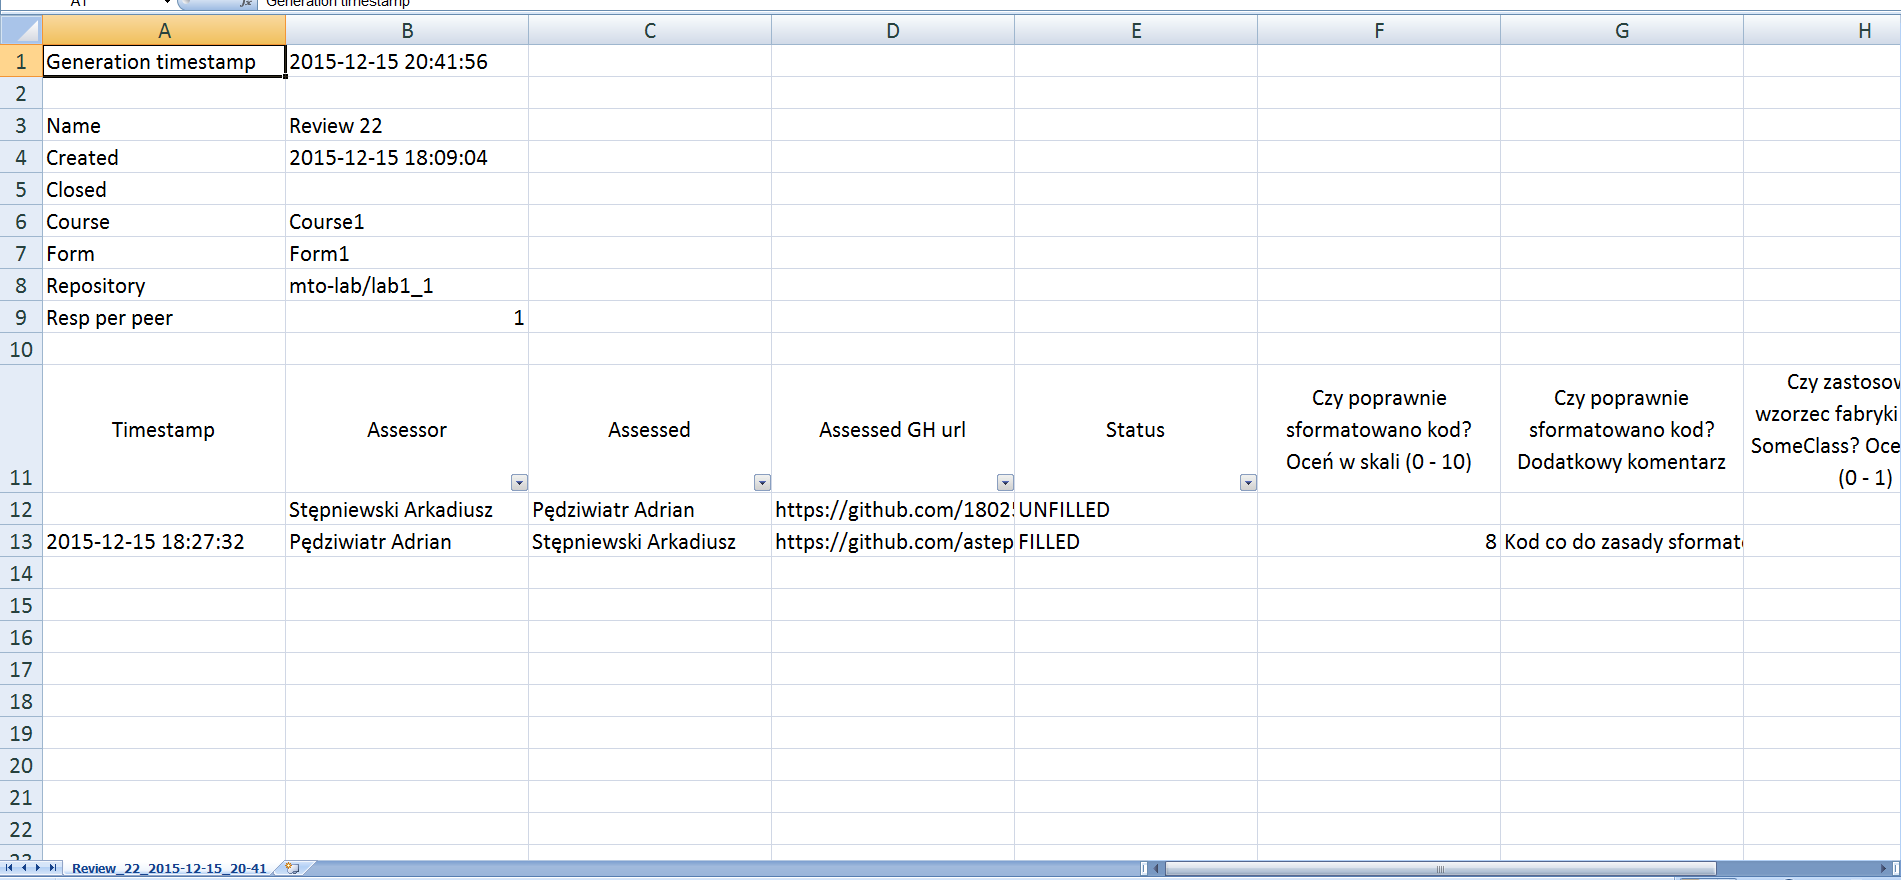
\includegraphics[width=\textwidth]{7_1excel}
    \caption{Zrzut ekranowy: arkusz MS Excel z~podsumowaniem dokonanych ocen}
    \label{obr71}
\end{figure}


\clearpage
\section{Statystyki systemu i~sprzątanie}
System posiada jeszcze jedną podstronę kontrolno-sprzątającą zaprezentowaną na rysunku \ref{obr81}. Znajdują się na niej informacje statystyczne i~techniczne (ściśle związane ze sposobem implementacji, mogą być pomocne przy rozwiązywaniu problemów). Wśród wypisywanych informacji są takie dane jak:
\begin{itemize}
    \item wykorzystanie aktualnego limitu połączeń z~GitHub API;
    \item stan pamięci podręcznej - czy jest ona włączona, oraz możliwość zmiany stanu;
    \item stan pamięci podręcznej - ilość wykorzystanego miejsca, oraz możliwość skasowania zapamiętanych informacji;
    \item procentowy wskaźnik udziału pamięci podręcznej przy wykonywaniu żądań http;
    \item przybliżona liczba zgłoszonych zadań związanych z~anonimizacją prac (dana techniczna);
    \item przybliżona liczba zadań, związanych z~anonimizacją prac, oczekują w~kolejce do wykonania (dana techniczna);
    \item liczba zleceń, które mają w~systemie status przetwarzanych;
    \item liczba repozytoriów (anonimowych kopii) na koncie \textquote{manekin} (dummy), które nie mają pokrycia w~bazie danych i~nie są potrzebne. Do tej liczby zaliczają się także kopie związane z~zamkniętymi przeglądami. W~tym miejscu istnieje możliwość usunięcia ich z~konta;
    \item liczba folderów w~katalogu tymczasowym (powinna być równa zero, jeżeli brak jest zadań w~kolejce) (dana techniczna).
\end{itemize}

\begin{figure}[!h]
    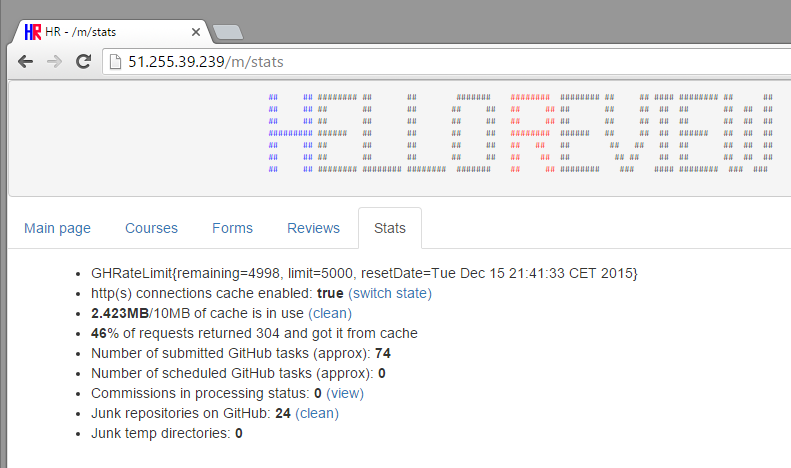
\includegraphics[width=400px]{8_1stats}
    \caption{Zrzut ekranowy: statystyki systemowe}
    \label{obr81}
\end{figure}


% ex: set tabstop=4 shiftwidth=4 softtabstop=4 noexpandtab fileformat=unix filetype=tex spelllang=pl,en spell:


    \chapter{Baza danych}

\section{Wstęp}
Dane wytwarzane przez system muszą być nieulotne. Z~tego powodu istnieje potrzeba składowania ich na dysku twardym. System zapisuje dane w~relacyjnej bazie danych zgodnej ze standardem SQL. 

\medskip
Wykorzystanym (i~skonfigurowanym) systemem zarządzania relacyjną bazą danych (ang. Relational Database Management System, RDBMS) jest H2 w~trybie wbudowanym (ang. embedded mode). Autor nie widzi potrzeby wykorzystania na potrzeby pracy inżynierskiej bazy danych w~trybie klient-server (ang. client-server mode). Zarówno wykorzystywany system bazy danych, jak i~tryb w~którym jest ona uruchomiana są konfigurowalne poprzez plik \textquote{application.properties}. Jeżeli zaistnieje potrzeba zmiany systemu zarządzania relacyjną bazą danych można to zrobić. Jedynym wymogiem jest, by była to baza relacyjna zgodna ze standardem SQL.

\medskip
Autor projektując bazę danych zastosował podejście \textquote{najpierw kod} (ang. code-first). Oznacza to, że autor zaprojektował bazę danych, jako zbiór encji (ang. entities) - klas języka Java zgodnych ze standardem mapowania relacyjno-obiektowego w~tym języku (tj. Java Persistence API, JPA). Za utworzenie odpowiednich tabel bazodanych, na podstawie istniejących encji, odpowiedzialny jest zastosowany silnik mapowania relacyjno-obiektowego - implementacja JPA - Hibernate. Dla każdej encji wspominany silnik utworzył odpowiadającą jej tabelę w~bazie danych.

\section{Schemat bazy danych}

\medskip
Rysunek \ref{diagram} na stronie \pageref{diagram} przedstawia zastosowany w~systemie schemat bazy danych. Rysunek ten zawiera tabele i~istniejące pomiędzy nimi powiązania. 

\begin{landscape}
\begin{figure}[!ht]
    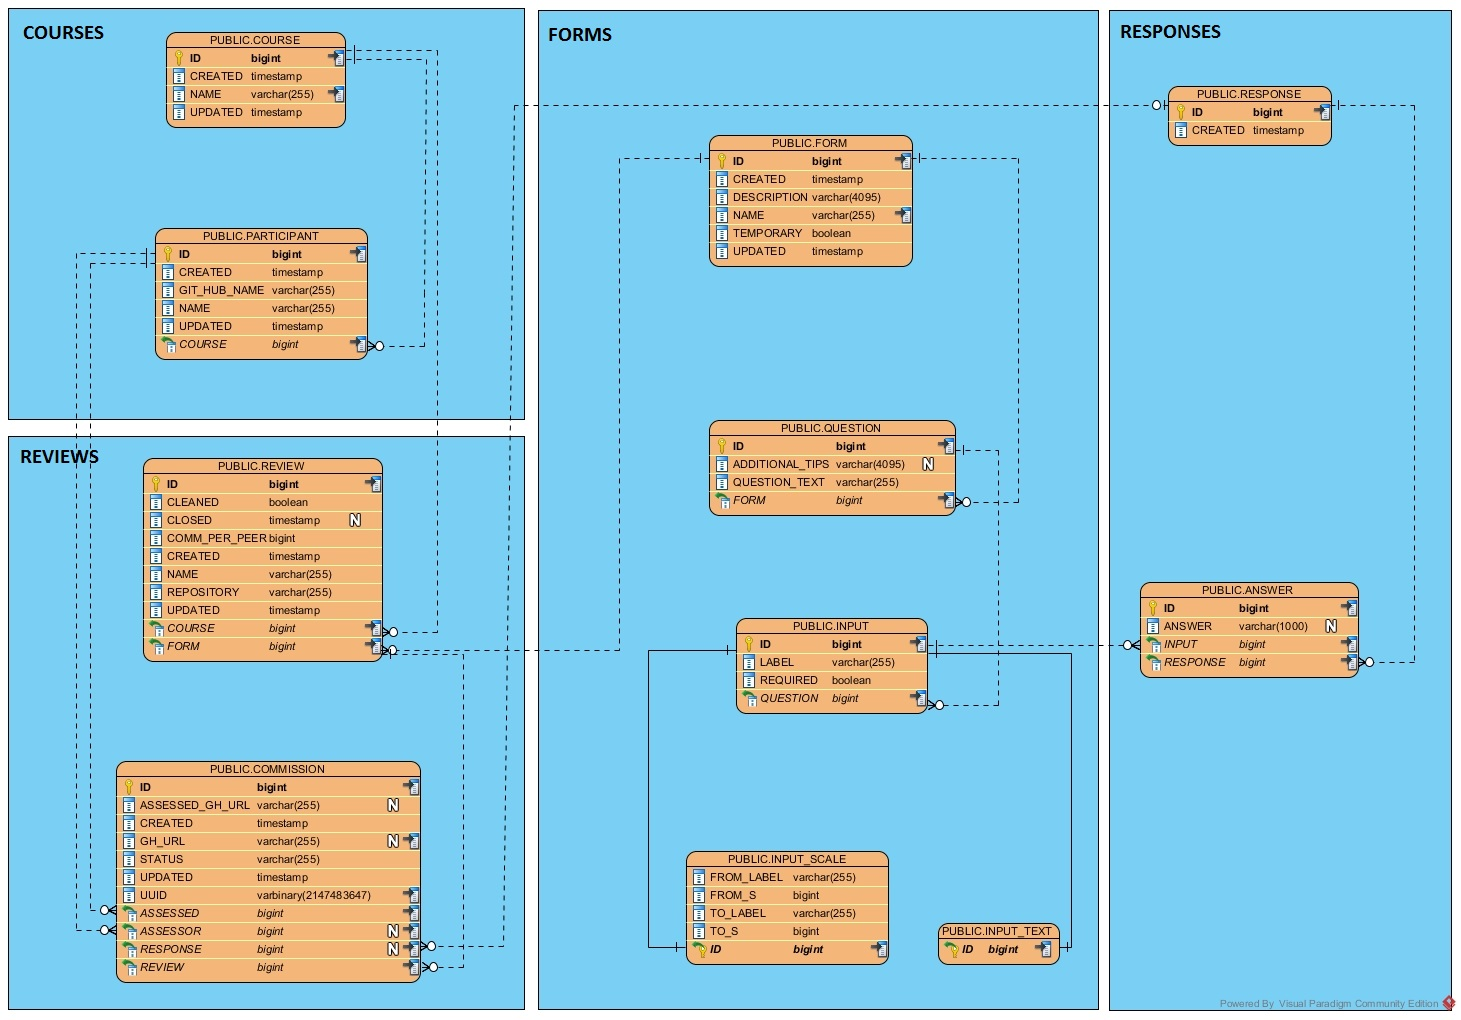
\includegraphics[width=600px]{diagram}
    \caption{Schemat bazy danych}
    \label{diagram}
\end{figure}
\end{landscape}

Autor podzielił model bazy danych na cztery części wzajemnie ze sobą powiązane:
\begin{enumerate}
    \item kursy (ang. courses) - encje odpowiedzialne za kursy i~uczestników;
    \item formularze (ang. forms) - encje odpowiedzialne za system formularzy;
    \item przeglądy (ang. review) - encje odpowiedzialne za przeglądy i~zlecenia;
    \item odpowiedzi (ang. responses) - encje odpowiedzialne za odpowiedzi na zlecenia przeglądów.
\end{enumerate}

\medskip
Cechą wspólną wszystkich encji jest to, że system zapisuje w~atrybutach czas ich utworzenia (\textquote{created}). Większość z~nich zawiera także czas ostatniej aktualizacji (\textquote{updated}). Czas aktualizacji nie jest notowany dla encji, które~z założenia są niemodyfikowalne (ang. immutable)~i nie będą zmieniane.

\subsection{Kursy}
Kursy zostały opisane przy użyciu dwóch encji. Pierwsza z~nich \textquote{course} odpowiada za przechowywanie informacji na temat utworzonych kursów - nadanej nazwy (\textquote{name}),. Druga z~encji to \textquote{participant} i~przechowuje informacje o~uczestnikach zapisanych do danego kursu - imię (\textquote{name}), nazwa konta w~usłudze GitHub (\textquote{githubname}).

\subsection{Formularze}
Każdy formularz posiada odpowiedni wpis w~encji \textquote{form}. Formularz charakteryzuje się nazwą (\textquote{name}). Zawiera także opis (\textquote{description)}, listę pytań (\textquote{question}) i~znacznikiem, czy jest to wpis tymczasowy (\textquote{temporary}). Wpis tymczasowy to atrybut związany z~zastosowaną implementacją podglądu formularza podczas jego tworzenia. Wpis oznaczony przez system jako tymczasowy nie może zostać użyty na innych etapach i~zostanie automatycznie usunięty przy najbliższej okazji.

\medskip
Pytania, które wchodzą w~skład formularza posiadają takie atrybuty jak: treść pytania (\textquote{question\textunderscore text}), opcjonalne informacje dodatkowe (\textquote{additional\textunderscore tips}). Pytanie zawiera także listę kontrolek (\textquote{input}), które mogą być typu skala (\textquote{input\textunderscore scale}) lub tekst (\textquote{input\textunderscore text}).

\subsection{Przeglądy}
Encje związane z~przeglądami to przegląd (\textquote{review}) i~zlecenie (\textquote{commission}). Przegląd jest ogólnym pojęciem i~jest związany z~grupą. Prowadzący zleca przegląd w~grupie. Przegląd może składać się z~wielu zleceń. Zlecenie jest to pojedyncze zadanie ocenienia pracy autorstwa kursanta A~przez innego kursanta B.

\medskip
\clearpage
Przegląd zawiera takie atrybuty jak:
\begin{itemize}
    \item nazwa (\textquote{name});
    \item nazwa źródłowego repozytorium z~ocenianym zadaniem (\textquote{repository});
    \item liczba zleceń w~ramach przeglądu przypadająca na jednego kursanta (\textquote{comm\textunderscore per\textunderscore peer});
    \item znacznik, czy przegląd został już zamknięty (\textquote{closed});
    \item odnośnik do zastosowanego formularza (\textquote{form});
    \item odnośnik do kursu dla którego przegląd został zlecony (\textquote{course}).
\end{itemize}

\medskip
Zlecenie zawiera następujące atrybuty:
\begin{itemize}
    \item odnośnik do przeglądu, do którego zlecenie nalęży (\textquote{review});
    \item odnośnik do kursanta, którego praca jest oceniania (\textquote{assessed});
    \item odnośnik do kursanta, który ma dokonać oceny (\textquote{assessor});
    \item adres URL do repozytorium z~ocenianą pracą (\textquote{assessed\textunderscore gh\textunderscore url});
    \item indywidualny numer przeglądu, zgodny ze standardem UUID4 (\textquote{uuid});
    \item status przeglądu (\textquote{status});
    \item odnośnik do udzielonej odpowiedzi (\textquote{response}).
\end{itemize}

\subsection{Odpowiedzi}
Każde zlecenie zawiera odnośnik do udzielonej odpowiedzi. Za przechowywanie odpowiedzi odpowiadają encje \textquote{response} i~\textquote{answer}. Pierwsza z~nich nie zawiera szczególnych atrybutów - jest to jedynie informacja, że odpowiedź została udzielona. Jedynym atrybutem jest czas udzielenia odpowiedzi (\textquote{created}).

\medskip
Dla każdej kontrolki, która była w~formularzu przypisanym do zlecenia, utworzony zostaje wpis typu \textquote{answer}. Encja taka zawiera odnośnik do kontrolki, której dotyczy (\textquote{input}), odpowiedź udzieloną przez kursanta (\textquote{answer}), oraz odnośnik do encji \textquote{response}, która identyfikuje zlecenie.

% ex: set tabstop=4 shiftwidth=4 softtabstop=4 noexpandtab fileformat=unix filetype=tex spelllang=pl,en spell:

    \chapter{Napotkane problemy w~implementacji}
Implementacja nigdy nie przebiega bezproblemowo. Rozdział ten przeznaczony został na opisanie najciekawszych napotkanych przez autora problemów w~trakcie realizacji tytułowego systemu, wraz z~genezą ich powstania i~sposobem dotarcia do przyczyny lub zastępczego rozwiązania.

\section{Wyjątki związane z połączeniem do GitHub API}
Autor użył do komunikacji z~GitHub API biblioteki autostwa Kohsuke Kawaguchi o~nazwie org.kohsuke:github-api. W~opinii autora reprezentacja obiektowa została w~niej przystępnie zaprojektowana i~jest ona prosta w~obsłudze. Okazało się jednak, że dla żądań listujących (np. lista powieleń repozytorium) w~przypadku niepowodzenia rzuca ona błędem typu \textquote{Error}, zamiast wyjątkiem typu \textquote{Exception} lub \textquote{RuntimeException}. Sytuację taką przedstawia listing na rysunku \ref{koderr1}. W~ocenie autora użycie takiego typu błędu nie jest odpowiednim rozwiązaniem oraz jest niepożądane dla działania systemu. Autor jako rozwiązanie napisał dodatkową klasę pomocniczą \textquote{GHExecutor}, która przetwarza wyjątki rzucane przez tą bibliotekę, na własny \textquote{GHCommunicationException} i~jednocześnie \textquote{zamienia} nieporządane błędy w~wyjątki. Listing napisanej klasy zawiera rysunek numer \ref{koderr2} na stronie \pageref{koderr2}. Wszystkie wywołania używanej biblioteki, które powodują połączenie z usługą GitHub zostały \textquote{opakowane} napisaną klasą użytkową.

\begin{figure}[!h]
\centering
    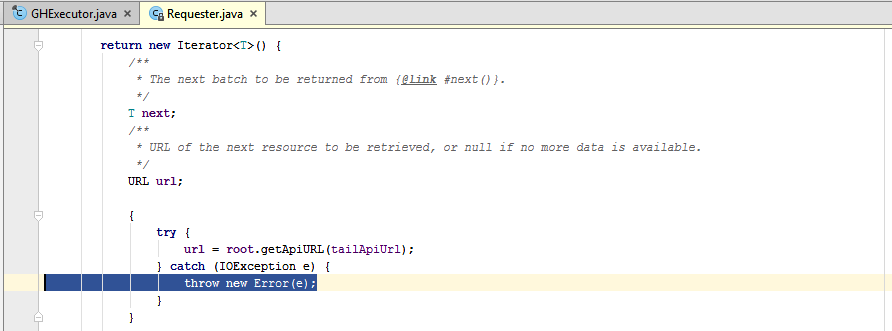
\includegraphics[width=400px]{kod_error1}
    \caption{Listing kodu źródłowego: nieoczekiwany błąd (Error) podczas połączeń z GitHub API}
    \label{koderr1}
\end{figure}


\begin{figure}[!h]
\centering
    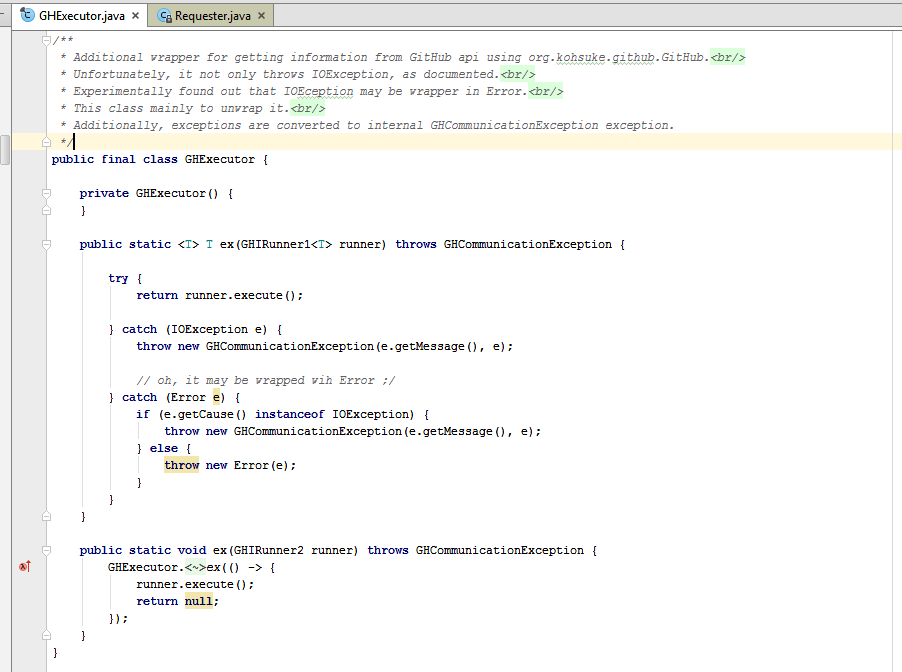
\includegraphics[width=\textwidth]{kod_error2}
    \caption{Listing kodu źródłowego: klasa GHCommunicationException}
    \label{koderr2}
\end{figure}

\section{Pamięć podręczna dla połączeń z~GitHub API}
Połączeń do GitHub API nie można wykonywać dowolnie dużo. GitHub limituje liczbę połączeń na godzinę. Limit ten dla połączeń anonimowych wynosi 60, natomiast dla połączeń używających danych autoryzacyjnych 5000 \cite{GitHubApiDoc}. Limit jest więc bardzo duży - wystarczy się przedstawić, a~można wysyłać zapytania o~zasoby częściej niż co sekundę. Teoretycznie można się nim nie przejmować limitem, i~nie wykonywać żadnych optymalizacji w~tym kierunku.

\medskip
Warto jednak pamiętać, że wykorzystujemy darmową usługę, i~chociażby w~ramach podziękowania zastosować się do wskazówek w~oficjalnej dokumentacji GitHub API. Znajduje się tam informacja, że jeżeli zapytania są wysyłane z~użyciem mechanizmów pamięci podręcznej, to w~ramach podziękowania w~pewnych przypadkach wykonanie zapytania nie obniża limitu. W~wielu odpowiedziach wysyłane są nagłówki HTTP \textquote{ETag} i/lub \textquote{Last-Modified}. Informacje te pozwalają wysłać żądanie warunkowe - \textquote{Podaj mi proszę zasób, tylko jeżeli się zmienił. W~przypadku braku zmian użyję odpowiedzi zapisanej w~pamięci podręcznej}. Jeżeli odpowiedzią na takie zapytanie warunkowe jest kod \textquote{304 Not Modified}, czyli \textquote{brak zmian}, to limit nie jest obniżany.

\medskip
Podążając wskazówkami autor postanowił dostosować swój kod, tak, by z~takiej pamięci podręcznej korzystał. W~dokumentacji biblioteki wykorzystywanej implementacji dostępu do GitHub API w~języku java - tj. \textquote{org.kohsuke: github-api}, znajduje się się rekomendacja zmiany domyślnego agenta http, na bibliotekę \textquote{OkHttp}, która obsługuje mechanizm pamięci podręcznej. Tak też zrobiono. Włączenie mechanizmu pamięci podręcznej spowodowało jednak, że algorytm kopiowania przestał działać poprawnie - nagle bardzo spowolnił, ilość zapytań paradoksalnie nie zmalała, a~wzrosła.

\medskip
Zapisywane informacje z~przebiegu działania algorytmu nie wskazywały jasno przyczyny. Ich analiza wykazała jednak, że przestój następował w~momencie odpytywania GitHub API o~informację, czy wysyłana gałąź w~repozytorium już jest widoczna jako zasób, co terminuje iż jej wysyłanie zakończyło się. Autor wysnuł teorię, że interfejs programistyczny usługi GitHub się myli, i~odpowiada niezgodnie z~rzeczywistością w~przypadku wysyłania zapytań warunkowych. Teoria ta znalazła potwierdzenie w~trakcie niezależnych prób z~użyciem ręcznie wysyłanych zapytań narzędziem cURL - okazało się, że zapytanie z~użyciem nagłówka \textquote{ETag} działa prawidłowo, ale dla \textquote{Last-Modified} informacja już jest błędna. Autor zgłosił błąd, a~programista GitHub potwierdził jego istnieje i~utworzenie w~wewnętrznym systemie zgłoszenia. Poinformował także, że nagłówek ten nie powinien być w~ogóle w~tym miejscu obsługiwany.

\medskip
Nie chcąc rezygnować z~pamięci podręcznej, w~tym momencie wydawało się jasne, że należy zmienić konfigurację biblioteki \textquote{OkHttp}, tak by dostosować priorytet używania nagłówków. Analiza dokumentacji i~kodu źródłowego tej biblioteki wykazała jednak, że obsługa nagłówka \textquote{ETag} ma priorytet przed nagłówkiem \textquote{Last-Modified}, więc wszystko powinno być w~porządku. Debugowanie aplikacji przy użyciu aplikacji Charles Proxy, tj. podsłuchując wykonywane połączenia HTTP w~systemie, wykazało, że prawdopodobnie GitHub API nie odpowiada nieprawidłowo. Właściwie to w~ogóle nie odpowiada, gdyż nie może - żadne zapytanie http nie zostało do niego wysłane.

\medskip
Ostatecznie okazało się, że GitHub API wysyła w~odpowiedzi nagłówek \textquote{Cache-Control: private, max-age=60, s-maxage=60}. Nagłówek ten informuje agenta http, że uzyskana odpowiedź pozostaje aktualna przez następne 60 sekund, i~nie ma powodu, by w~tym czasie wysyłać to zapytanie jeszcze raz. Używany agent http - OkHttp - prawidłowo obsługuje ten nagłówek, i~dostając żądanie o~ten sam zasób w~ciągu 60 sekund od jego zapamiętania, w~ogóle nie wykonuje połączenia, tylko od razu pobiera informację z~pamięci podręcznej. Dla algorytmu kopiującego informacja sprzed kilku sekund nie jest świeża, należy bezwzględnie zapytać o~aktualność zasobu dostawcę, tj. usługę GitHub. Nadpisanie tego nagłówka własną wartością rozwiązało problem.

\medskip
Debugując ten problem autor zupełnie przez przypadek znalazł błąd w~interfejsie programistycznym usługi GitHub. Błąd, chociaż istnieje, nie miał wpływu na faktyczną przyczynę spowolnienia algorytmu. Jest to ciekawe doświadczenie ukazujące, że nawet starannie wykonany zapis przebiegu działania algorytmu nie zawsze dostarcza poszukiwanej informacji. Nie oznacza to jednak, że takich zapisów nie należy dokonywać - bardzo ułatwiają one debugowanie aplikacji, a~przetoczoną historię należy traktować w~kategorii wyjątku potwierdzającego regułę.

\section{Relacja dziedziczenia po stronie bazy danych}
Inny warty zanotowania problem autor znalazł w~trakcie implementacji systemu formularzy. Jest to błąd z~kategorii heisenbug (za Wikipedia: \textquote{rodzaj błędu programu komputerowego, który wymyka się próbom wyizolowania warunków jego występowania, na przykład nie występuje lub daje inne rezultaty w~trakcie próby powtórzenia go w~tych samych warunkach} \cite{Heisenbug}).

\medskip
Moduł odpowiedzialny z~formularze operuje między innymi na takich encjach jak: Question, Input, InputText, InputScale. Question jest encją odpowiedzialną za przechowywanie szczegółów danego pytania, pozostaje ona w~relacji jeden do wielu z~encją Input. Encja Input natomiast jest typem abstrakcyjnym - przechowuje informacje wspólne dla wszystkich typów dostępnych form odpowiedzi. Encje InputText i~InputScale uszczegóławiają ten typ abstrakcyjny, i~są odpowiedzialne za konkretne typy formy odpowiedzi: odpowiednio komentarz tekstowy, i~ocena w~skali.

\medskip
Problem wynika z~połączenia wczytywania leniwego (ang. lazy) i~relacji dziedziczenia po stronie bazy danych. Z~jakiegoś powodu w~jednym z~miejsc otrzymywany typ Input wyrażał jedynie abstrakcyjną encję Input, nie był natomiast żadnym z~typów szczegółowych. Próba debugowania tego błędu była niemożliwa - ustawienie punktu stopu naprawiało problem - otrzymywany Input był typu szczegółowego.  Autor nie znalazł przyczyny takiego zachowania, nie wiadomo dlaczego w~trakcie próby debugowania błąd nie istniał. Nie może być to błąd typu race conditition, gdyż problem dotyczy otrzymanego typu otrzymanego obiektu.

\medskip
Pierwszą dokonaną próbą naprawy sytuacji było wyłączenie odczytu leniwego z~bazy, i~zastąpienie go chciwym (ang. eager). Mimo, że jest to bardzo skuteczne rozwiązania, to wyjątkowo słabe. Ilość dokonywanych zapytań do bazy danych diametralnie wzrosła. Taki spadek wydajności nie był do zaakceptowania.

\medskip
Ostatecznie problem został ominięty poprzez wykonanie inicjalizacji obiektu i~dokonanie jego konwersji na typ \textquote{prawdziwy}, zamiast operować na obiekcie typu \textquote{proxy} dostarczanego przez silnik dokonujący mapowania relacyjno-obiektowego. Zmiana ta została dodana do akcesora listy encji tupu Input w~encji Question. Po tej zmianie system działa prawidłowo, i~relacja dziedziczenia nie dostarcza problemów. Nie jest to jednak wyjaśnienie dlaczego bez tego występują problemy, i~gdzie faktycznie znajduje się błąd. Próba powtórzenia na prostszym, minimalistycznym projekcie się nie powiodła. Autor zrezygnował z~poszukiwania źródeł problemu z~ramach wykonywania pracy inżynierskiej, zastosowane rozwiązanie uznał za zadowalające.


% ex: set tabstop=4 shiftwidth=4 softtabstop=4 noexpandtab fileformat=unix filetype=tex spelllang=pl,en spell:

    \chapter{Możliwe kierunki rozwoju systemu}

Przygotowany system jest kompletny. Wszystkie założone wymagania znajdują pokrycie w~zrealizowanej funkcjonalności. Nie oznacza to jednak, że nie można go rozbudowywać i~rozszerzać dostępnych możliwości. Poniżej wymieniono kilka wartych rozważenia opcji wraz z~próbą przybliżenia stopnia trudności ich realizacji. 

\section{Internacjonalizacja}
System komunikuje się z~użytkownikiem w~języku angielskim. Umożliwienie komunikacji w~innym języku jest relatywnie proste. Należy przetłumaczyć komunikaty, które zostały już zebrane w~jednym pliku, oraz zaprogramować funkcję zmiany języka komunikatów w~interfejsie (front-end). Funkcjonalność taka została przewidziana na serwerze (back-end), i~odpowiednie funkcje po tej stronie są gotowe do użycia.

\medskip
Inaczej jest jednak z~systemem formularzy, za pomocą którego recenzent udziela odpowiedzi. Ten system nie został zaprojektowany z~myślą o~wyświetlaniu komunikatów w~wielu językach. Nie stanowi to problemu, jeżeli kurs składa się w~całości z~osób komunikujących się jednym wspólnym językiem. Formularz pod konkretne zadanie można utworzyć wielokrotnie - za każdym razem wpisując komunikaty w~języku odpowiednim dla danego kursu. Możliwość tworzenia wielonarodowościowych kursów nie została przewidziana i~wymaga przebudowy systemu formularzy.

\section{Wielu prowadzących}
System umożliwia ustawienie uprawnień master (prowadzący) wielu użytkownikom. Wszyscy jednak mają tą samą listę kursów, formularzy,  zleceń i~recenzji. Elementy te nie mają przypisanego właściciela i~wymagają wspólnego zaufania pomiędzy osobami z~uprawnieniami prowadzącego. Podczas projektowania nie została przewidziana taka możliwość, więc logika z~tym związana nie istnieje. Należy ją dopisać, co spowoduje także wymóg zmiany struktury bazodanowej. 

\section{Ręczny przydział przeglądów}
Prowadzący przy zlecaniu przeglądu może określić ile prac każdy z~kursantów powinien ocenić. Jest to obecnie realizowane losowo, z~uwzględnieniem równomierności przydziału, i~braku możliwości oceny swojej pracy. Nie ma jednak możliwości ręcznego przydziału kto czyją pracę powinien ocenić. Realizacja takiej opcji nie powinna sprawiać problemów komplementacyjnych, choć wymaga dostosowania algorytmu do takiej możliwości.

\section{Panel konfiguracyjny}
System obecnie jest konfigurowany przy użyciu pliku XML. Konfiguracja jest ładowana raz - przy uruchomieniu serwera. Nie ma możliwości zmiany konfiguracji podczas działania systemu. Zmiana zawartości pliku konfiguracyjnego wymaga przeładowania całego systemu. System można usprawnić umożliwiając zmianę konfiguracji podczas pracy systemu. Sposobów na realizację tego są co najmniej dwa. Jednym z~nich jest zrealizowanie opcji ponownego odczytu konfiguracji, i~aktualizacji elementów zależnych od tej konfiguracji podczas działania systemu - przy czym nadal konfiguracja znajduje się pliku. Drugim sposobem jest przebudowanie systemu konfiguracji na nowo - wprowadzenie panelu konfiguracyjnego, i~przeniesienie wpisów konfiguracyjnych z~pliku do systemu bazodanowego.

\medskip
Stopień skomplikowania zależy od przyjętych nowych założeń, które elementy konfiguracji mogą być zmienione bez potrzeby ponownego uruchomienia serwera. Niektóre z~nich nie sprawią żadnych trudności, i~nie wymagają dodatkowych działań. Do nich zaliczyć można np. listę osób z~uprawnieniami prowadzących, czy listę kont, które są źródłem zadań w~usłudze Github. Są jednak też takie, których zmiana może znacznie skomplikować logikę. Do tych zaliczyć należy zmianę folderu, który służy jako cache połączeń, oraz zmianę sekretnych danych OAuth2 identyfikujących aplikację w~usłudze GitHub. 

\section{Obsługa repozytoriów prywatnych}
System zrealizowano bazując na obsłudze kont darmowych - w~których repozytoria kontroli wersji są publicznie dostępne. Wykorzystana usługa GitHub umożliwia jednak także tworzenie organizacji w~ramach których repozytoria są prywatne. Konta takie zwykle są płatne, lecz w~tym konkretnym przypadku można poprosić o~licencję akademicką, do celów naukowych. Aktualnie takie repozytoria nie są obsługiwane.

\medskip
GitHub API repozytorium, i~repozytorium w~ramach organizacji uznaje za inny rodzaj zasobu. Ten drugi nie jest w~tym momencie w~ogóle używany. Algorytmy należy uogólnić, tak by odpytywał o~prawidłowy zasób. Należy też rozbudować konfigurację systemu i~formularz tworzenia zleceń przeglądów.

\section{Zmniejszenie ilości wykonywanych kopii}
Zastosowany algorytm anonimizacji można zoptymalizować pod kątem czasowym, ilości wykonywanych operacji, i~zapytań do GitHub API. Miejscem, w~którym można znaleźć dość oczywisty słaby punkt jest ilość wykonywanych kopii. W~tym momencie, jeżeli w~ramach przeglądu prowadzący kurs zleci, by każdy ocenił pracę 3 innych kolegów, to każda z~prac będzie skopiowana co najmniej 3 razy - dla każdej oceny.

\medskip
Usunięcie wykonywania zbędnych kopii wymaga kilku zmian. Po pierwsze, najbardziej oczywiste - poprawa algorytmu kopiującego. Po drugie zmiana struktury bazodanowej - która aktualnie przewiduje oddzielny link dla każdej kopii. Do takiej zmiany dostosować należało by także algorytmy oczyszczające - kasujące kopie, tak by nie próbowały wielokrotnie usuwać tego samego repozytorium.


% ex: set tabstop=4 shiftwidth=4 softtabstop=4 noexpandtab fileformat=unix filetype=tex spelllang=pl,en spell:

    \chapter{Podsumowanie}

W ocenie autora realizacja systemu zakończyła się sukcesem. Udało się zaprojektować, zaimplementować i~opisać działający system, który spełnia wszystkie założone wymagania. System może być wdrożony i~używany. Dzięki wysokiej integracji z~repozytoriami Git i~usługą GitHub system nie jest zamkniętym ekosystemem, którego wykorzystanie wymaga zmiany przyzwyczajeń prowadzących. Studenci mogą oceniać wykonanie zadania przez kolegów, na zlecenie prowadzącego, nie sugerując się autorem rozwiązania. Poszerzą w~ten sposób swoją wiedzę oraz będą pisać kod coraz wyższej jakości. Autor głęboko wierzy w~biznesową użyteczność stworzonego narzędzia i~korzyści jakie może przynieść jego wykorzystanie.
    
    \thispagestyle{empty}
    \listoffigures
    
    \nocite{*}
    \printbibliography[title={Bibliografia}]
    
\end{document}

% ex: set tabstop=4 shiftwidth=4 softtabstop=4 noexpandtab fileformat=unix filetype=tex spelllang=pl,en spell:
